


% \section{Extended Topology Scalability Details and Visual Results}
% \label{appendix:extended}
% \secReview


% This appendix presents the methodological details and extended analysis supporting the scalability experiments described in Section~\ref{sec:Coordination_section}, along with the complete visualization results for all network sizes and tasks. While the main paper focuses on comparative performance outcomes and high-level insights, the content here expands on the internal mechanics of convergence, failure formation, and negotiation dynamics at the agent level.

% \paragraph{Evaluation Structure and Experimental Conditions.}
% All experiments maintain a fixed LLM configuration, unified prompt template, and shared termination criteria across topologies. This standardization ensures that performance differences reflect communication topology rather than model variance. Each topology is evaluated for scalability and structural sensitivity under increasing agent count, specifically at network sizes $n \in \{4, 8, 16, 50, 100\}$, enabling observation of small-network reasoning efficiency and high-scale degradation. For every run, we measure success rate, convergence rounds, runtime overhead, and token consumption, emphasizing how topology modifies system stability as scale increases.

% \paragraph{Rounds-to-Convergence Rule.}
% For bounded tasks such as \textsc{Coloring}, \textsc{Matching}, and \textsc{VertexCover}, convergence proceeds within a predefined round limit. For global agreement tasks (\textsc{Consensus}, \textsc{LeaderElection}) and for settings where $n > 16$, we instead define the maximum convergence horizon as \(T = 2D + 1,\) where $D$ denotes the network diameter. This bound guarantees full information diffusion and aligns with classical distributed agreement theory. Under this rule, several high-scale runs exceed the nominal eight-round budget, occasionally requiring fifteen to nineteen rounds depending on the communication diameter of the topology.

% \paragraph{Matching Score Formulation.}
% Matching accuracy is evaluated through node-level reciprocal agreement. A match is considered valid if an agent selects a neighbor and that neighbor selects the agent in return; nonreciprocal or invalid choices produce inconsistent assignments. The final score is therefore computed as \(\text{Score} = 1 - \frac{\text{InconsistentNodes}}{|V|}.\) The visual outputs highlight reciprocal edges in green, one-directional matches in orange, inconsistent nodes in red, and unused edges in gray. This representation exposes the negotiation structure and illustrates failure propagation patterns even when global numeric scores appear moderate.

% \paragraph{Topology-Dependent Failure Dynamics.}
% Different network structures exhibit distinct breakdown mechanisms. Small-World graphs communicate rapidly through clustered connectivity and cross-cutting long links, producing reliable convergence at moderate scale. Scale-Free topologies achieve high stability when hub nodes coordinate successfully, but failure cascades occur when hubs diverge. Delaunay graphs emphasize geometric locality, increasing communication diameter and frequently yielding fragmented partial consensus at scale. CrewAI hierarchical orchestration accelerates symmetry resolution for leader-based coordination but is less robust under distributed allocation and multi-conflict tasks. Fully-connected Star communication behaves like a shared broadcast medium, achieving strong global consensus with small rounds and tokens usage.


% \subsection{Visualization-Driven Interpretation}
% \label{appendix:visualization}

% The following figures present the complete output visualizations across all tasks, topologys, and network sizes. They illustrate not only success or failure outcomes, but also reveal \emph{why} topologys diverge as the number of agents increases and how errors propagate during negotiation.

% \paragraph{Consensus (Figure~\ref{fig:consensus-results}).}
% Green regions indicate complete agreement, while red areas represent conflicting beliefs. Star retains unified global consensus across all scales. WS and BA maintain partial coherence until approximately $n=50$, after which divergence pockets emerge. Delaunay networks exhibit visibly isolated red clusters at large scale, directly corresponding to the sharp performance decline observed in Section~\ref{sec:Coordination_section}.

% \paragraph{Coloring (Figure~\ref{fig:coloring-results}).}
% Green edges indicate conflict-free adjacency, while red denotes color collisions. Scale-Free maintains stable chromatic separation through hub diffusion, whereas Delaunay produces localized red density as neighborhood isolation deepens. CrewAI-Sequential often reaches early convergence but not necessarily optimal partitions.

% \paragraph{Matching (Figures~\ref{fig:matching-results}–~\ref{fig:matching-results-modified}).}
% Figure~\ref{fig:matching-results} depicts full pairing structure, while Figure~\ref{fig:matching-results-modified} expands this into local reciprocal state representation. Green edges mark mutual matches, orange reflects one-sided selection, red nodes denote inconsistency, and gray edges represent unused adjacency. LangGraph-BA remains stable up to mid-scale, whereas Delaunay degenerates into dense orange-red instability webs at larger network sizes.

% \paragraph{LeaderElection (Figure~\ref{fig:leader-results}).}
% Green nodes mark the elected leader, red indicates competing leader clusters, and gray denotes followers. Hierarchical CrewAI consistently produces a single stable leader even at $n=100$, while WS and BA often spawn competing leadership pockets when scaled.

% \paragraph{VertexCover (Figure~\ref{fig:vertexcover-results}).}
% Green nodes indicate valid minimal coverage, blue represents non-minimal but correct membership, orange marks incorrect selections, and red edges highlight uncovered graph links. Small-World and Scale-Free converge toward compact covers, whereas Delaunay and hierarchical variants frequently over-cover or leave edge violations beyond fifty nodes.


% \subsection{Cross-Task Scalability Summary}
% \label{appendix:summary}

% Across all results and visual evidence, three dominant patterns emerge. First, topologies with fast diffusion such as WS and BA consistently outperform geometric Delaunay structures under load. Second, hierarchical reasoning excels in symmetry-breaking tasks such as \textsc{LeaderElection} but struggles in allocation problems requiring high-conflict negotiation. Third, centralized broadcast structures (Star/All-to-All) achieve strong consensus but incur heavy communication cost, confirming that scalability and communication depth are tightly coupled. Together, these results establish a comprehensive picture of how multi-agent frameworks scale, where they converge, and under which structures they fail.






% 
\begin{figure*}[t]
    \centering
    % --- Row 1 ---
    \subfloat[SW ($n=4$)]{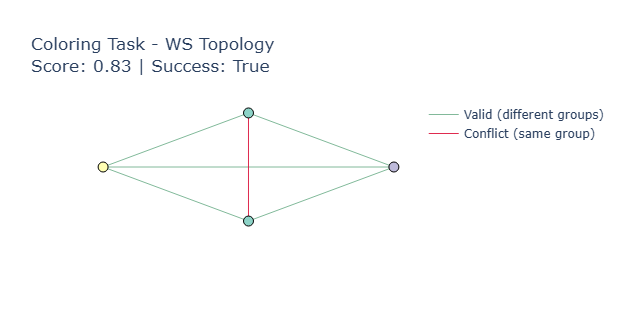
\includegraphics[trim=90 80 200 100,clip,width=0.12\textwidth]{figures/topology/coloring_results_20250917_222432_rounds8_gpt-4o-mini_nodes4.png}}
    \subfloat[SW ($n=8$)]{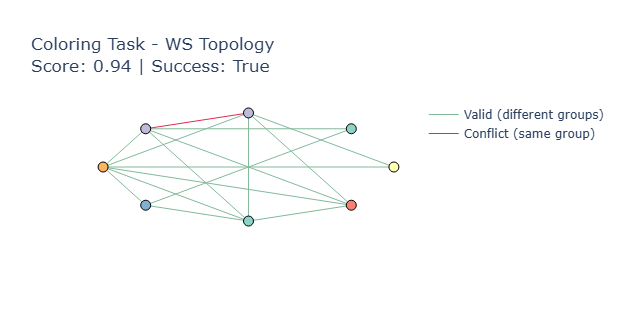
\includegraphics[trim=90 80 200 100,clip,width=0.16\textwidth]{figures/topology/coloring_results_20250917_222635_rounds8_gpt-4o-mini_nodes8.png}}
    \subfloat[SW ($n=16$)]{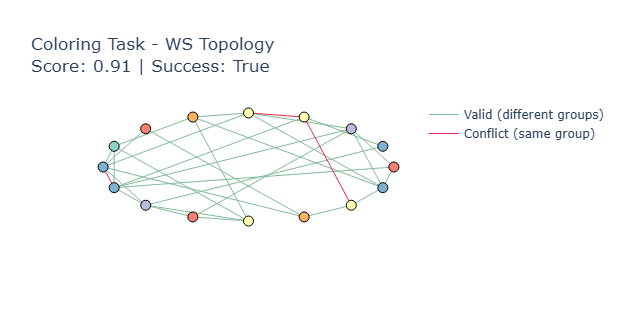
\includegraphics[trim=90 80 200 100,clip,width=0.19\textwidth]{figures/topology/coloring_results_20250917_222842_rounds8_gpt-4o-mini_nodes16.png}}
    \subfloat[SW ($n=50$)]{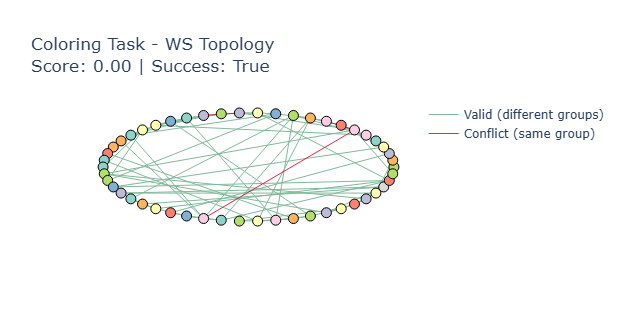
\includegraphics[trim=90 80 200 100,clip,width=0.22\textwidth]{figures/topology/coloring_results_20250920_135347_rounds11_gpt-4o-mini_nodes50.png}}
    \subfloat[SW ($n=100$)]{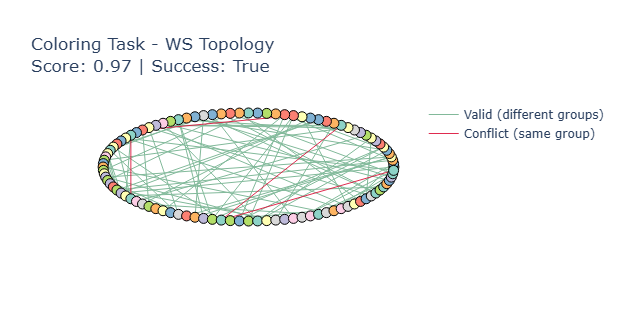
\includegraphics[trim=90 80 200 100,clip,width=0.26\textwidth]{figures/topology/coloring_results_20250920_141018_rounds15_gpt-4o-mini_nodes100.png}}

    % --- Row 2 ---
    \subfloat[SF ($n=4$)]{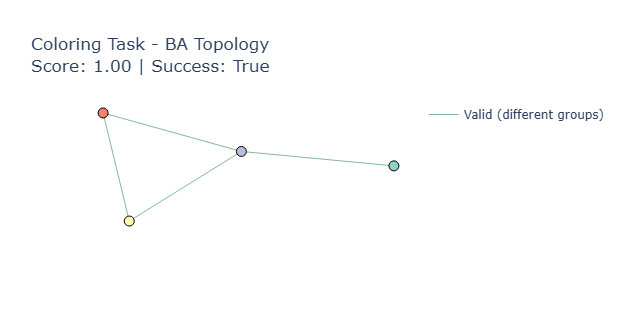
\includegraphics[trim=90 80 200 100,clip,width=0.12\textwidth]{figures/topology/coloring_results_20250917_223003_rounds8_gpt-4o-mini_nodes4.png}}
    \subfloat[SF ($n=8$)]{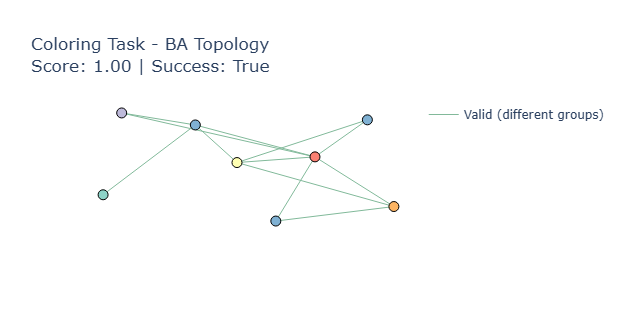
\includegraphics[trim=90 80 200 100,clip,width=0.16\textwidth]{figures/topology/coloring_results_20250917_223205_rounds8_gpt-4o-mini_nodes8.png}} 
    \subfloat[SF ($n=16$)]{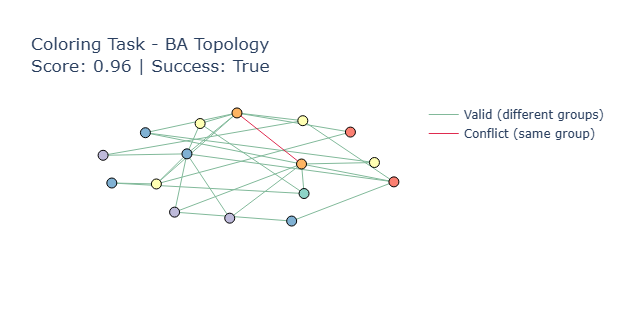
\includegraphics[trim=90 80 200 100,clip,width=0.19\textwidth]{figures/topology/coloring_results_20250917_223421_rounds8_gpt-4o-mini_nodes16.png}}
    \subfloat[SF ($n=50$)]{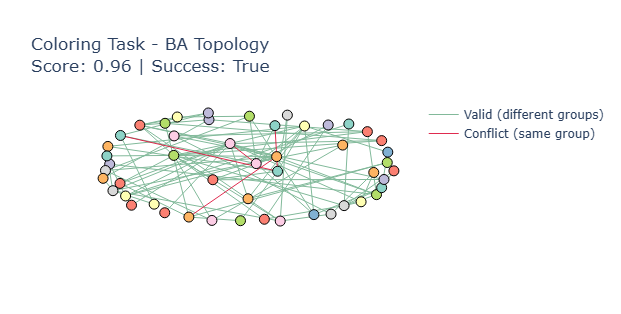
\includegraphics[trim=90 80 200 100,clip,width=0.22\textwidth]{figures/topology/coloring_results_20250920_141717_rounds11_gpt-4o-mini_nodes50.png}}
    \subfloat[SF ($n=100$)]{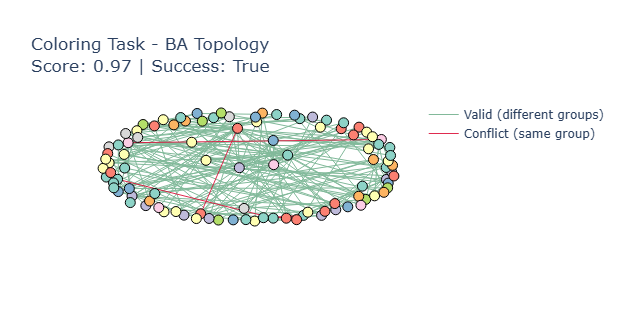
\includegraphics[trim=90 80 200 100,clip,width=0.26\textwidth]{figures/topology/coloring_results_20250920_142903_rounds11_gpt-4o-mini_nodes100.png}}

    % --- Row 3 ---
    \subfloat[DT ($n=4$)]{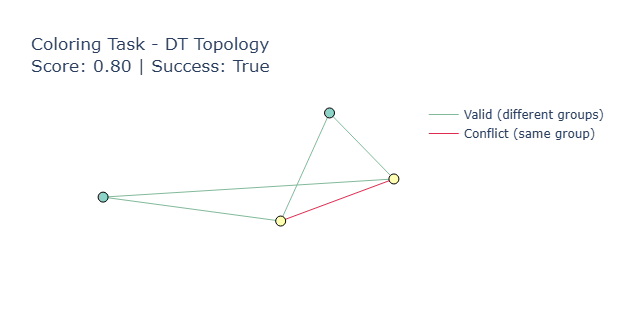
\includegraphics[trim=90 80 200 100,clip,width=0.12\textwidth]{figures/topology/coloring_results_20250917_223636_rounds8_gpt-4o-mini_nodes4.png}}
    \subfloat[DT ($n=8$)]{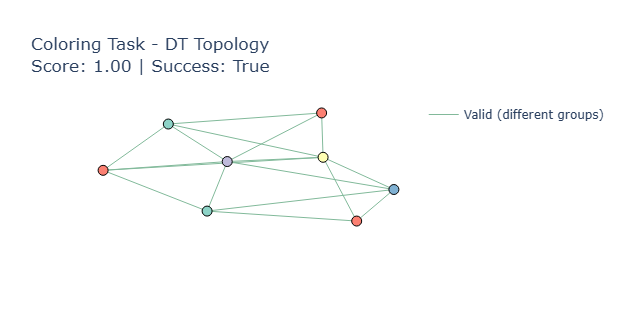
\includegraphics[trim=90 80 200 100,clip,width=0.16\textwidth]{figures/topology/coloring_results_20250917_223854_rounds8_gpt-4o-mini_nodes8.png}}
    \subfloat[DT ($n=16$)]{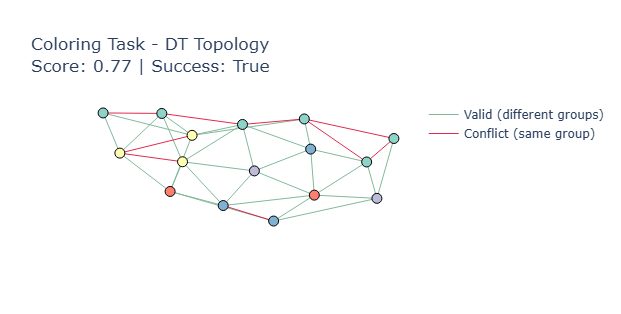
\includegraphics[trim=90 80 200 100,clip,width=0.19\textwidth]{figures/topology/coloring_results_20250917_224151_rounds8_gpt-4o-mini_nodes16.png}} 
    \subfloat[DT ($n=50$)]{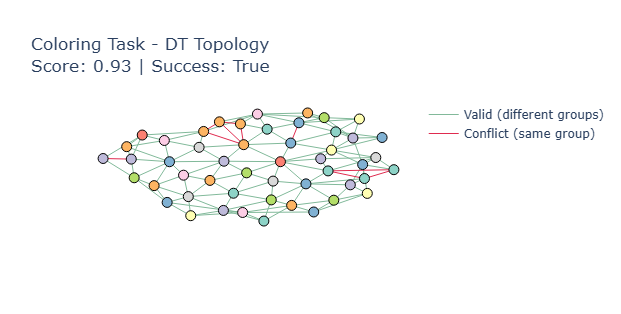
\includegraphics[trim=90 80 200 100,clip,width=0.22\textwidth]{figures/topology/coloring_results_20250920_143802_rounds13_gpt-4o-mini_nodes50.png}} 
    \subfloat[DT ($n=100$)]{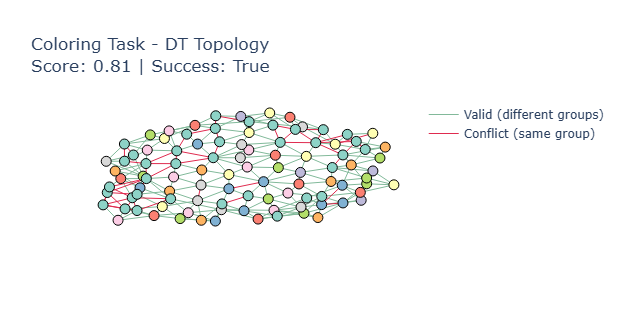
\includegraphics[trim=90 80 200 100,clip,width=0.26\textwidth]{figures/topology/coloring_results_20250920_145919_rounds19_gpt-4o-mini_nodes100.png}} \\



    \vspace{2mm}
    % --- Row 4 ---
    \subfloat[Seq. ($n=4$)]{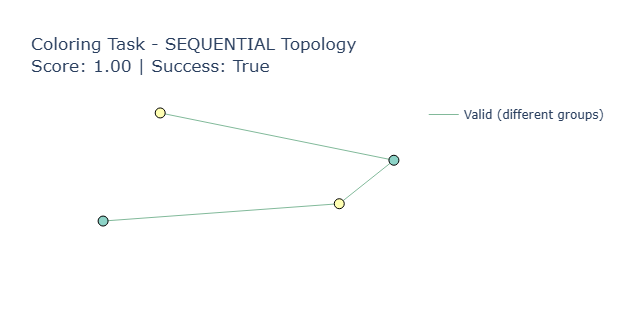
\includegraphics[trim=90 80 200 100,clip,width=0.12\textwidth]{figures/topology/coloring_results_20250924_130551_rounds8_gpt-4o-mini_nodes4.png}}
    \subfloat[Seq. ($n=8$)]{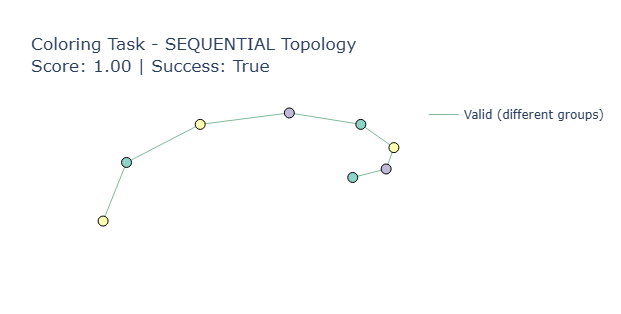
\includegraphics[trim=90 80 200 100,clip,width=0.16\textwidth]{figures/topology/coloring_results_20250924_130747_rounds8_gpt-4o-mini_nodes8.png}}
    \subfloat[Seq. ($n=16$)]{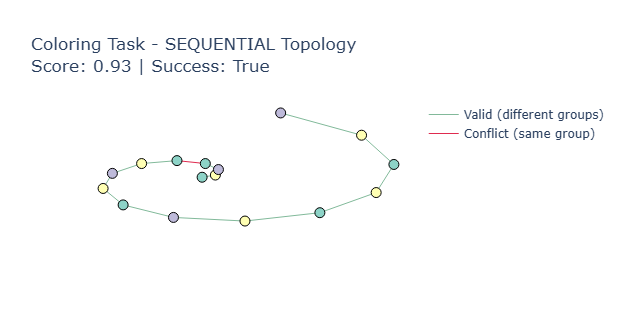
\includegraphics[trim=90 80 200 100,clip,width=0.19\textwidth]{figures/topology/coloring_results_20250924_131004_rounds8_gpt-4o-mini_nodes16.png}} 
    \subfloat{\rule{0.22\textwidth}{0pt}} % placeholder without number
    \subfloat{\rule{0.26\textwidth}{0pt}} % placeholder without number



    % --- Row 5 ---
    \subfloat[Hier. ($n=4$)]{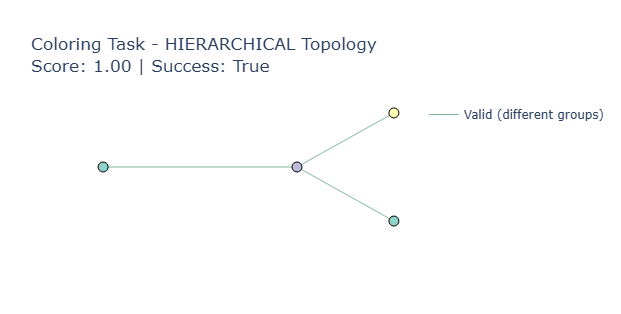
\includegraphics[trim=90 80 200 100,clip,width=0.12\textwidth]{figures/topology/coloring_results_20250924_143605_rounds8_gpt-4o-mini_nodes4.png}}
    \subfloat[Hier. ($n=8$)]{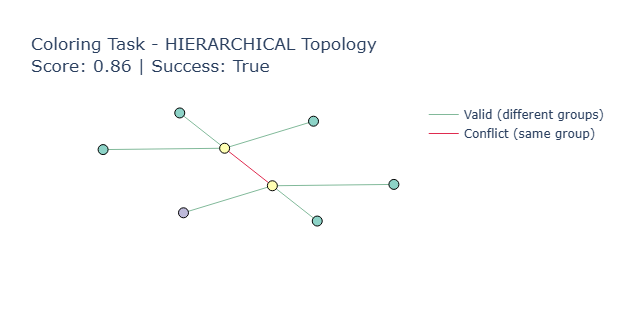
\includegraphics[trim=90 80 200 100,clip,width=0.16\textwidth]{figures/topology/coloring_results_20250924_143802_rounds8_gpt-4o-mini_nodes8.png}}
    \subfloat[Hier. ($n=16$)]{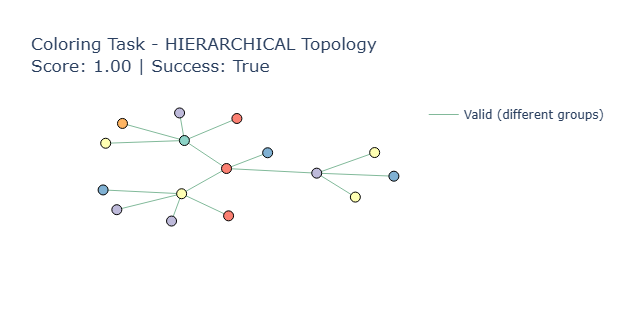
\includegraphics[trim=90 80 200 100,clip,width=0.19\textwidth]{figures/topology/coloring_results_20250924_144052_rounds8_gpt-4o-mini_nodes16.png}} 
    \subfloat[Hier. ($n=50$)]{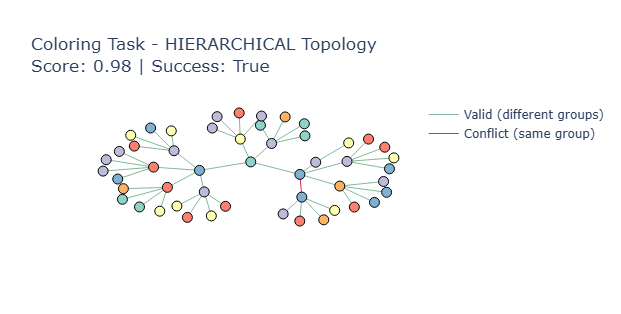
\includegraphics[trim=90 80 200 100,clip,width=0.22\textwidth]{figures/topology/coloring_results_20250924_235040_rounds13_gpt-4o-mini_nodes50}} 
    \subfloat[Hier. ($n=100$)]{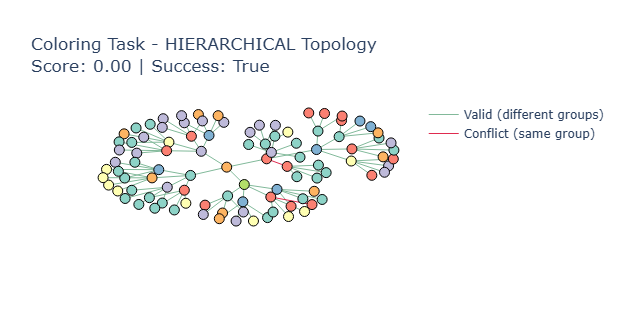
\includegraphics[trim=90 80 200 100,clip,width=0.26\textwidth]{figures/topology/coloring_results_20250925_000609_rounds15_gpt-4o-mini_nodes100}} \\

    \caption{Coloring experiment outcomes across different network sizes ($n=4$ to $100$). 
    Each subfigure shows the final group assignments of agents. 
    Valid assignments (neighbors in different groups) are shown in green, while conflicts (neighbors in the same group) are shown in red.}
    \label{fig:coloring-results}
\end{figure*}

% \begin{figure*}[t]
    \centering
    % --- WS ---
    \subfloat[SW ($n=4$)]{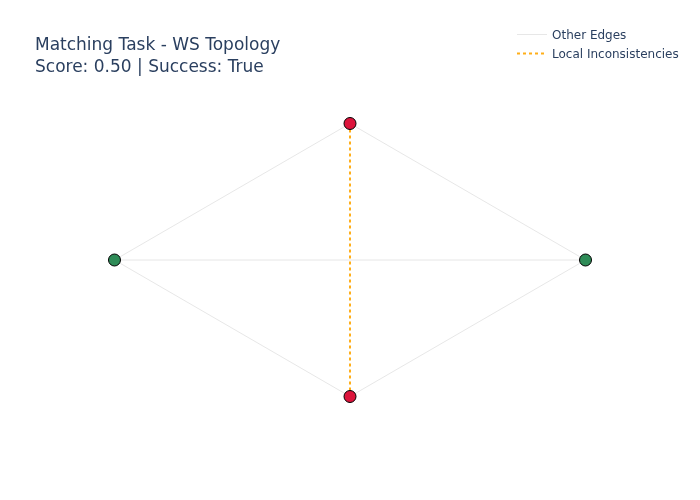
\includegraphics[trim=100 100 90 100,clip,width=0.12\textwidth]{figures/topology/matching_results_20250917_224359_rounds8_gpt-4o-mini_nodes4_langgraph_matching_original.png}}
    \subfloat[SW ($n=8$)]{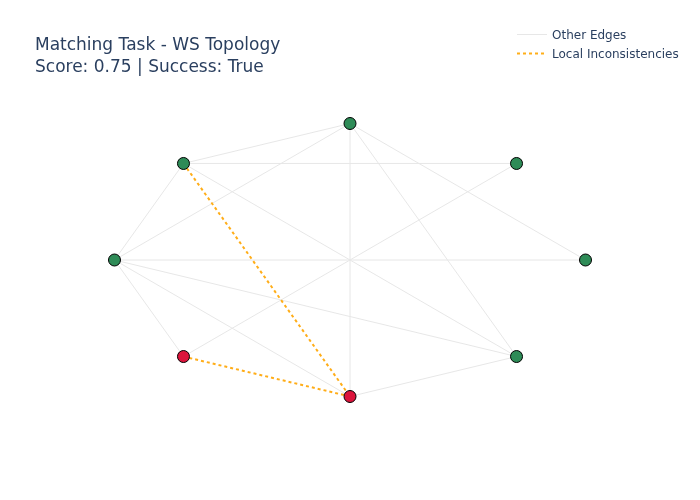
\includegraphics[trim=100 100 90 100,clip,width=0.16\textwidth]{figures/topology/matching_results_20250917_224622_rounds8_gpt-4o-mini_nodes8_langgraph_matching_original.png}}
    \subfloat[SW ($n=16$)]{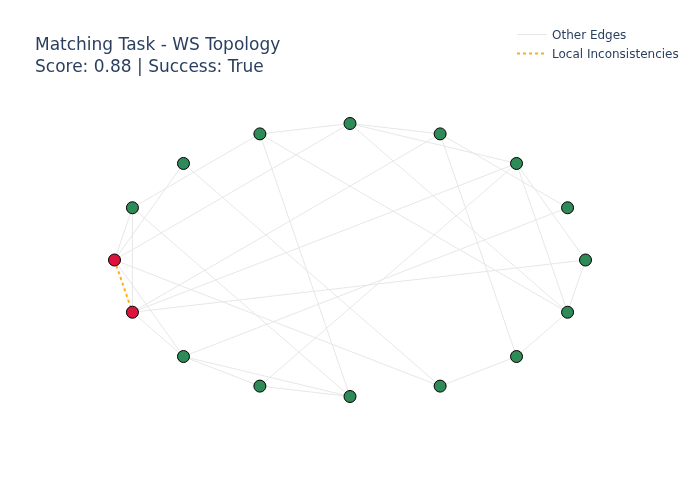
\includegraphics[trim=100 100 90 100,clip,width=0.19\textwidth]{figures/topology/matching_results_20250917_224907_rounds8_gpt-4o-mini_nodes16_langgraph_matching_original.png}}
    \subfloat[SW ($n=50$)]{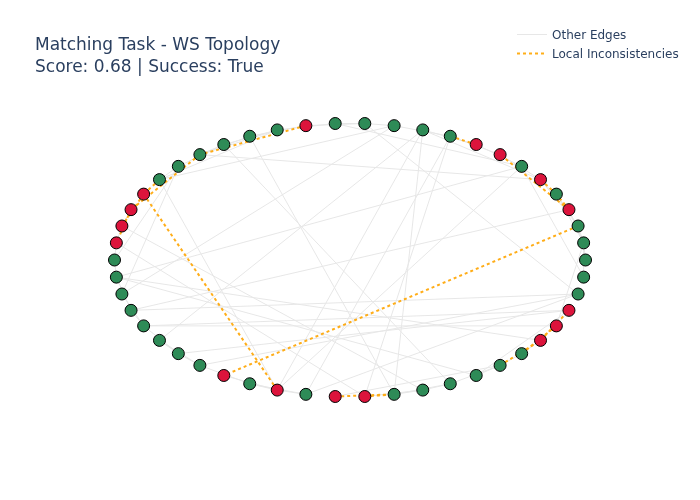
\includegraphics[trim=100 100 90 100,clip,width=0.22\textwidth]{figures/topology/matching_results_20250920_223026_rounds11_gpt-4o-mini_nodes50_langgraph_matching_original.png}}
    \subfloat[SW ($n=100$)]{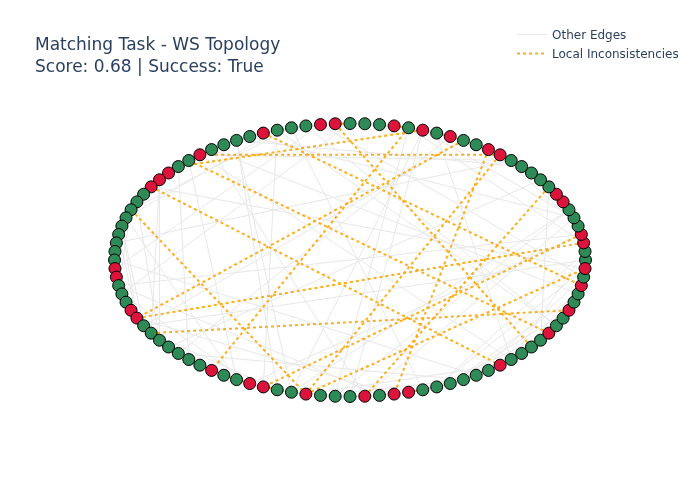
\includegraphics[trim=100 100 90 100,clip,width=0.26\textwidth]{figures/topology/matching_results_20250919_123428_rounds15_gpt-4o-mini_nodes100_langgraph_matching_original.png}}
    \\
    \vspace{2mm}
    % --- BA ---
    \subfloat[SF ($n=4$)]{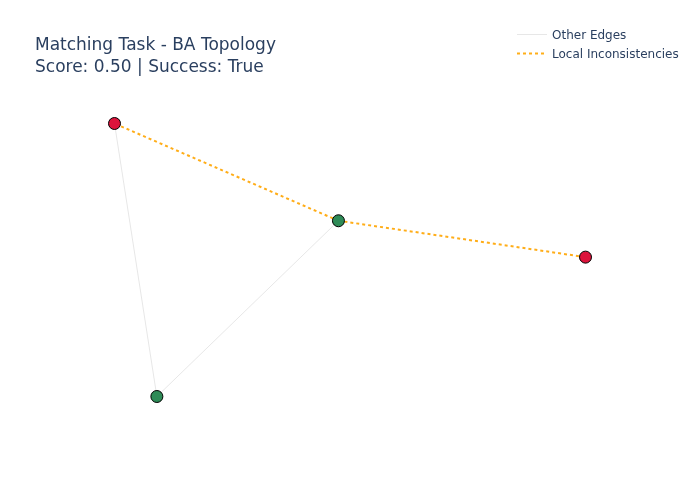
\includegraphics[trim=100 100 90 100,clip,width=0.12\textwidth]{figures/topology/matching_results_20250917_225048_rounds8_gpt-4o-mini_nodes4_langgraph_matching_original.png}}
    \subfloat[SF ($n=8$)]{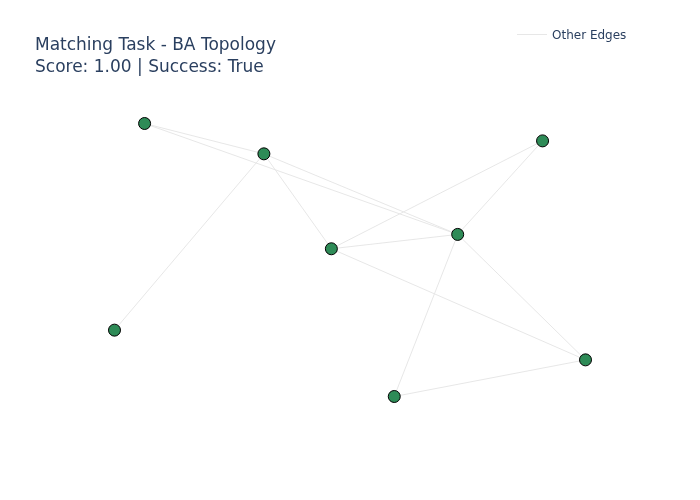
\includegraphics[trim=100 100 90 100,clip,width=0.16\textwidth]{figures/topology/matching_results_20250917_225237_rounds8_gpt-4o-mini_nodes8_langgraph_matching_original.png}}
    \subfloat[SF ($n=16$)]{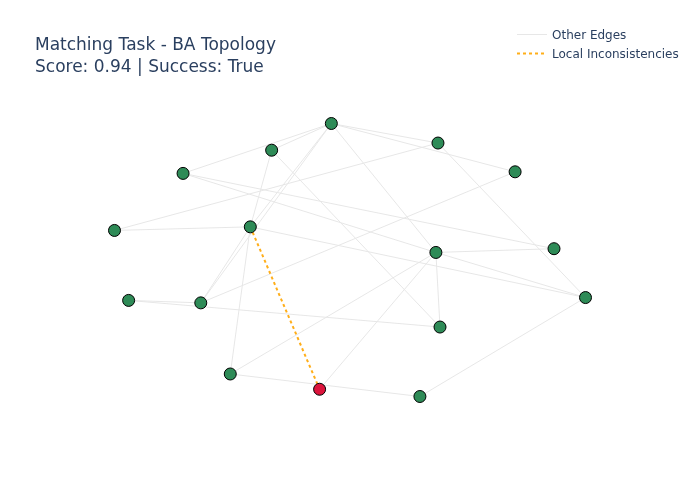
\includegraphics[trim=100 100 90 100,clip,width=0.19\textwidth]{figures/topology/matching_results_20250917_225456_rounds8_gpt-4o-mini_nodes16_langgraph_matching_original.png}}
    \subfloat[SF ($n=50$)]{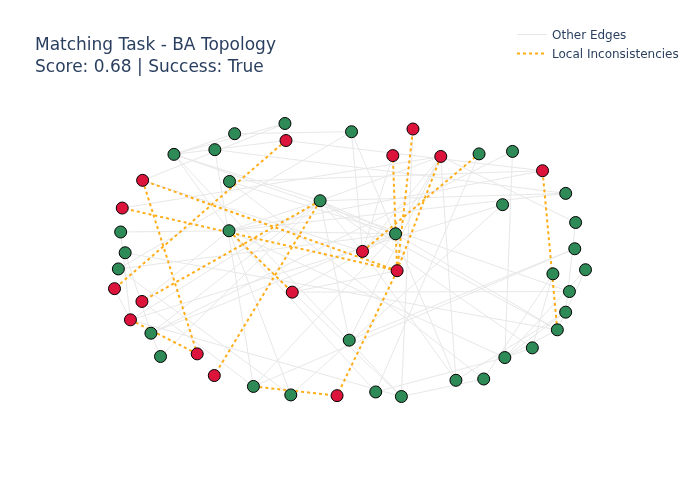
\includegraphics[trim=100 100 90 100,clip,width=0.22\textwidth]{figures/topology/matching_results_20250920_180551_rounds11_gpt-4o-mini_nodes50_langgraph_matching_original.png}}
    \subfloat[SF ($n=100$)]{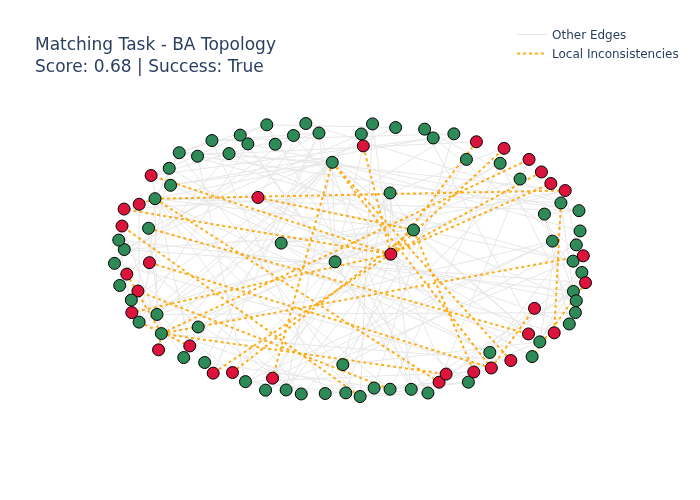
\includegraphics[trim=100 100 90 100,clip,width=0.26\textwidth]{figures/topology/matching_results_20250920_181618_rounds11_gpt-4o-mini_nodes100_langgraph_matching_original.png}}
    \\
    \vspace{2mm}
    % --- DT ---
    \subfloat[DT ($n=4$)]{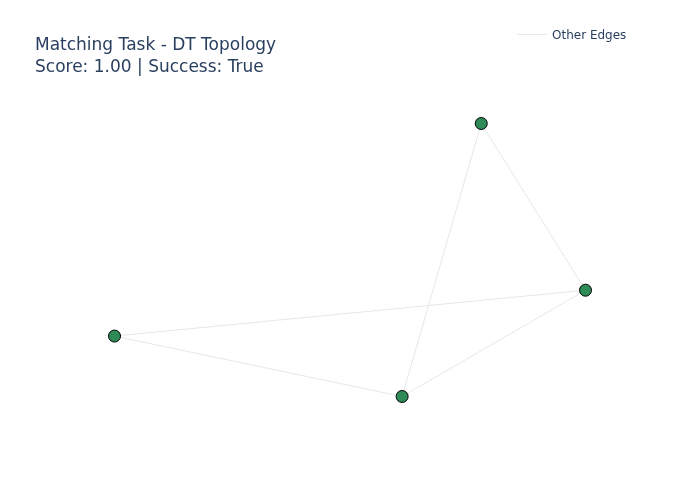
\includegraphics[trim=100 100 90 100,clip,width=0.12\textwidth]{figures/topology/matching_results_20250917_225625_rounds8_gpt-4o-mini_nodes4_langgraph_matching_original.png}}
    \subfloat[DT ($n=8$)]{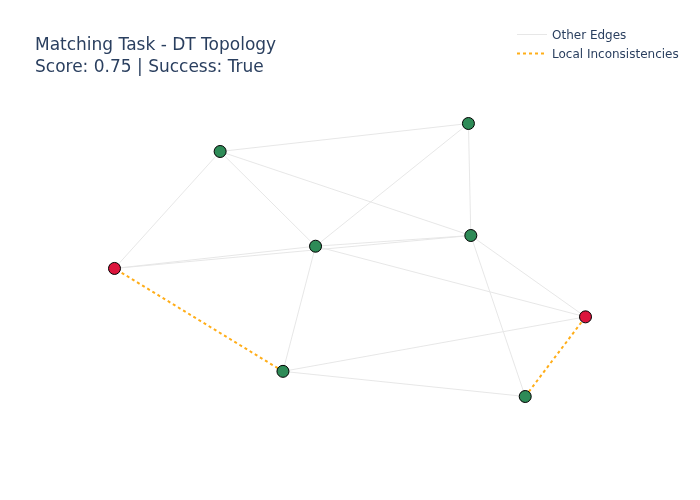
\includegraphics[trim=100 100 90 100,clip,width=0.16\textwidth]{figures/topology/matching_results_20250917_225759_rounds8_gpt-4o-mini_nodes8_langgraph_matching_original.png}}
    \subfloat[DT ($n=16$)]{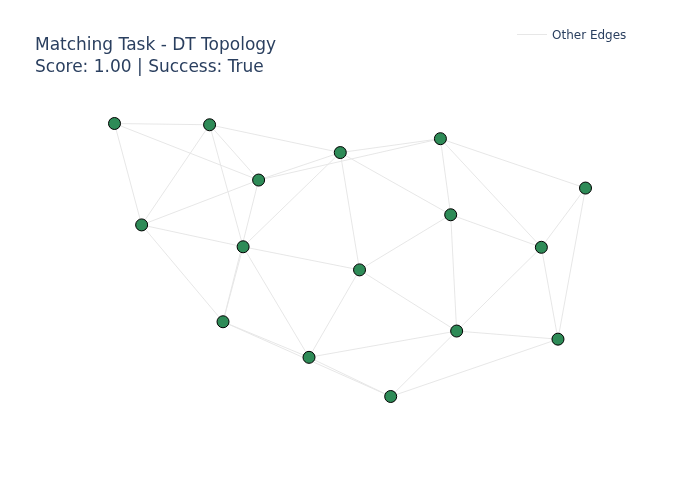
\includegraphics[trim=100 100 90 100,clip,width=0.19\textwidth]{figures/topology/matching_results_20250917_230008_rounds8_gpt-4o-mini_nodes16_langgraph_matching_original.png}}
    \subfloat[DT ($n=50$)]{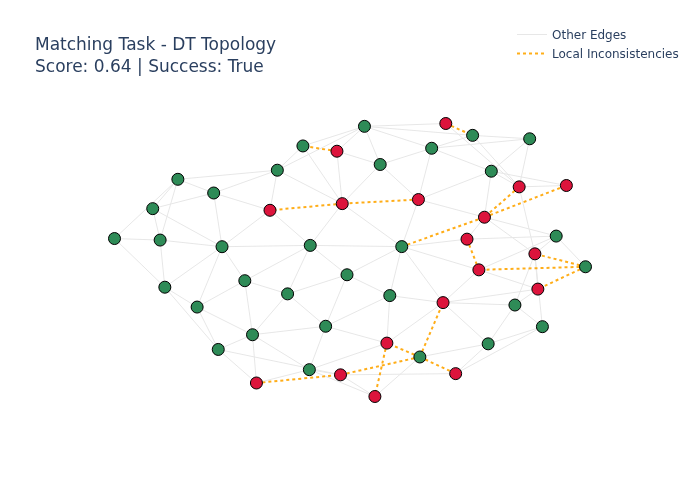
\includegraphics[trim=100 100 90 100,clip,width=0.22\textwidth]{figures/topology/matching_results_20250920_182438_rounds13_gpt-4o-mini_nodes50_langgraph_matching_original.png}}
    \subfloat[DT ($n=100$)]{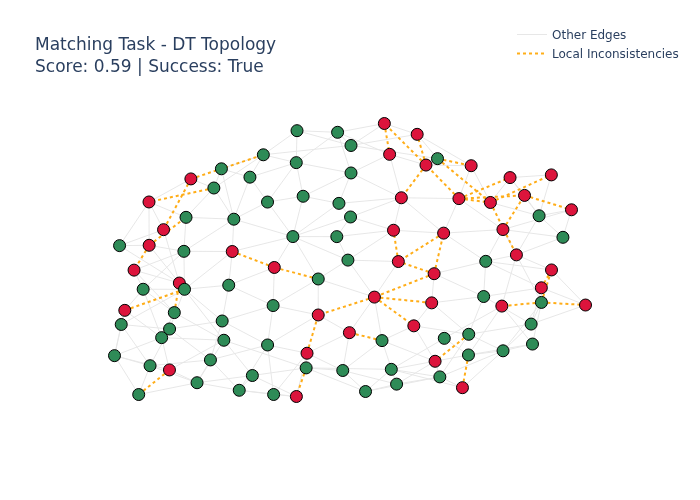
\includegraphics[trim=100 100 90 100,clip,width=0.26\textwidth]{figures/topology/matching_results_20250920_184622_rounds19_gpt-4o-mini_nodes100_langgraph_matching_original.png}}
    \\
    \vspace{2mm}
    % --- SEQUENTIAL ---
    \subfloat[Seq. ($n=4$)]{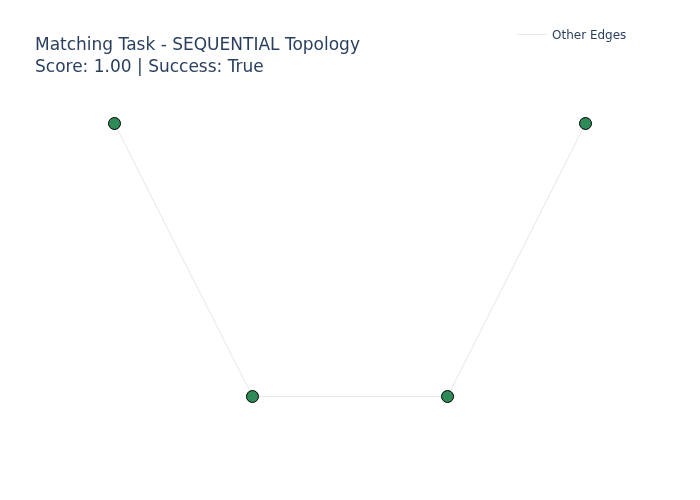
\includegraphics[trim=100 100 90 100,clip,width=0.12\textwidth]{figures/topology/matching_results_20250924_134419_rounds8_gpt-4o-mini_nodes4_crewai-sequential_matching_original.png}}
    \subfloat[Seq. ($n=8$)]{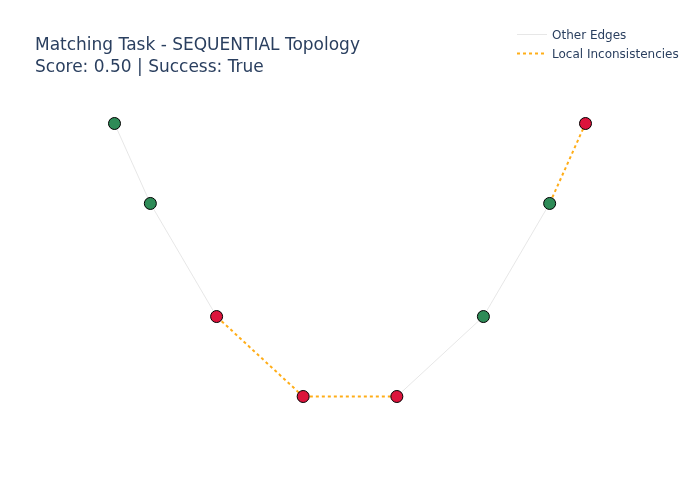
\includegraphics[trim=100 100 90 100,clip,width=0.16\textwidth]{figures/topology/matching_results_20250924_134606_rounds8_gpt-4o-mini_nodes8_crewai-sequential_matching_original.png}}
    \subfloat[Seq. ($n=16$)]{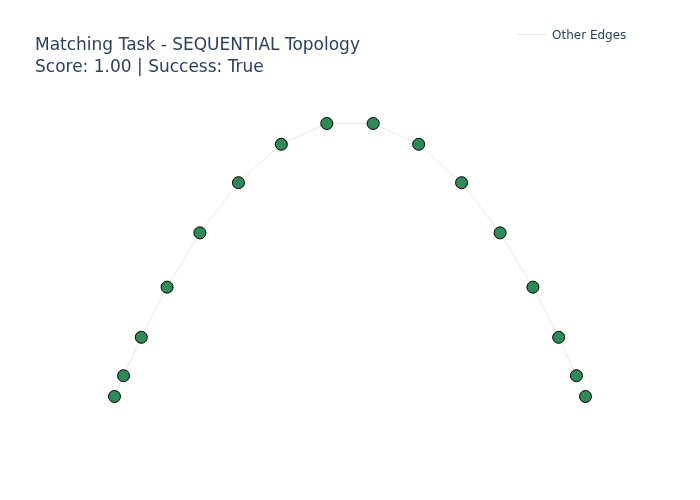
\includegraphics[trim=100 100 90 100,clip,width=0.19\textwidth]{figures/topology/matching_results_20250924_134833_rounds8_gpt-4o-mini_nodes16_crewai-sequential_matching_original.png}}
    \subfloat{\rule{0.22\textwidth}{0pt}} % placeholder without number
    \subfloat{\rule{0.26\textwidth}{0pt}} % placeholder without number
    \\
    \vspace{2mm}
    % --- HIERARCHICAL ---
    \subfloat[Hier. ($n=4$)]{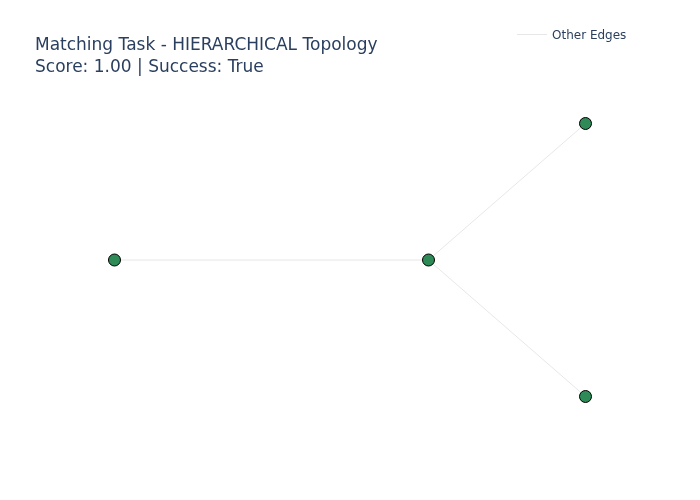
\includegraphics[trim=100 100 90 100,clip,width=0.12\textwidth]{figures/topology/matching_results_20250924_144228_rounds8_gpt-4o-mini_nodes4_crewai-hierarchical_matching_original.png}}
    \subfloat[Hier. ($n=8$)]{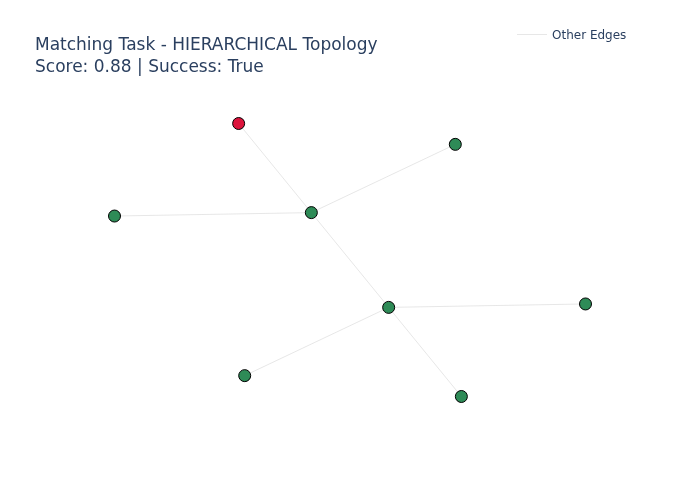
\includegraphics[trim=100 100 90 100,clip,width=0.16\textwidth]{figures/topology/matching_results_20250924_144411_rounds8_gpt-4o-mini_nodes8_crewai-hierarchical_matching_original.png}}
    \subfloat[Hier. ($n=16$)]{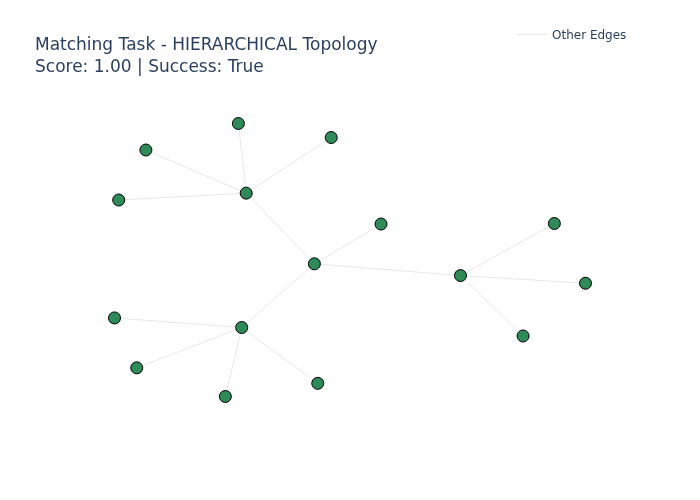
\includegraphics[trim=100 100 90 100,clip,width=0.19\textwidth]{figures/topology/matching_results_20250924_144629_rounds8_gpt-4o-mini_nodes16_crewai-hierarchical_matching_original.png}}
    \subfloat[Hier. ($n=50$)]{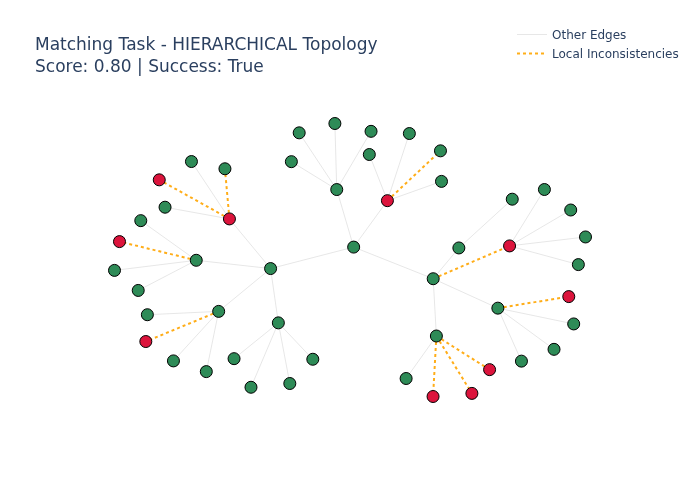
\includegraphics[trim=100 100 90 100,clip,width=0.22\textwidth]{figures/topology/matching_results_20250925_001343_rounds13_gpt-4o-mini_nodes50_crewai-hierarchical_matching_original.png}}
    \subfloat[Hier. ($n=100$)]{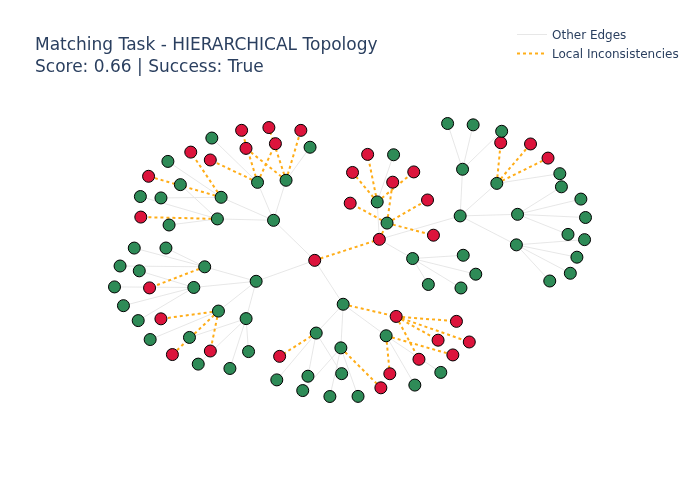
\includegraphics[trim=100 100 90 100,clip,width=0.26\textwidth]{figures/topology/matching_results_20250925_002721_rounds15_gpt-4o-mini_nodes100_crewai-hierarchical_matching_original.png}}
    \\
    \vspace{2mm}
    % --- ALL ---
    \subfloat[All ($n=4$)]{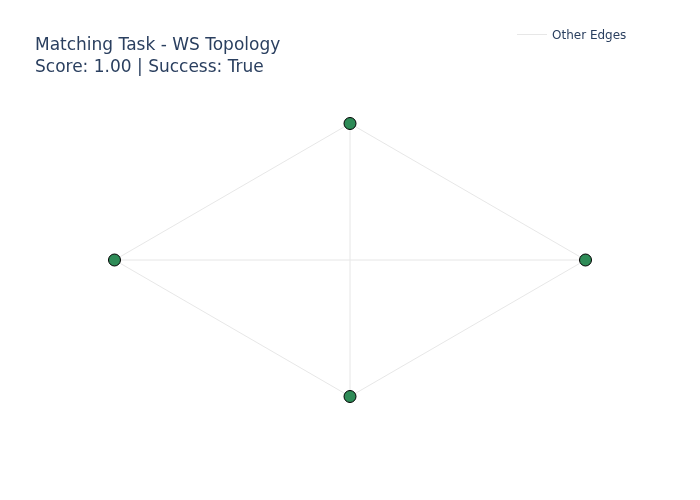
\includegraphics[trim=100 100 90 100,clip,width=0.12\textwidth]{figures/topology/matching_results_20250917_230141_rounds8_gpt-4o-mini_nodes4_concordia_matching_original.png}}
    \subfloat[All ($n=8$)]{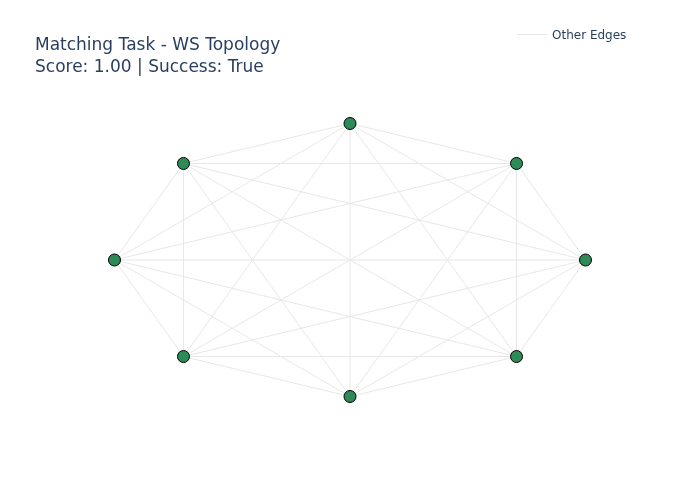
\includegraphics[trim=100 100 90 100,clip,width=0.16\textwidth]{figures/topology/matching_results_20250917_230411_rounds8_gpt-4o-mini_nodes8_concordia_matching_original.png}}
    \subfloat[All ($n=16$)]{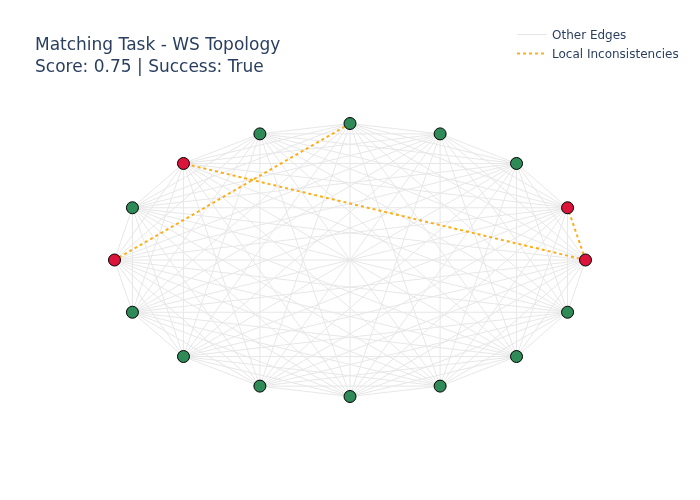
\includegraphics[trim=100 100 90 100,clip,width=0.19\textwidth]{figures/topology/matching_results_20250917_230756_rounds8_gpt-4o-mini_nodes16_concordia_matching_original.png}}
    \subfloat[All ($n=50$)]{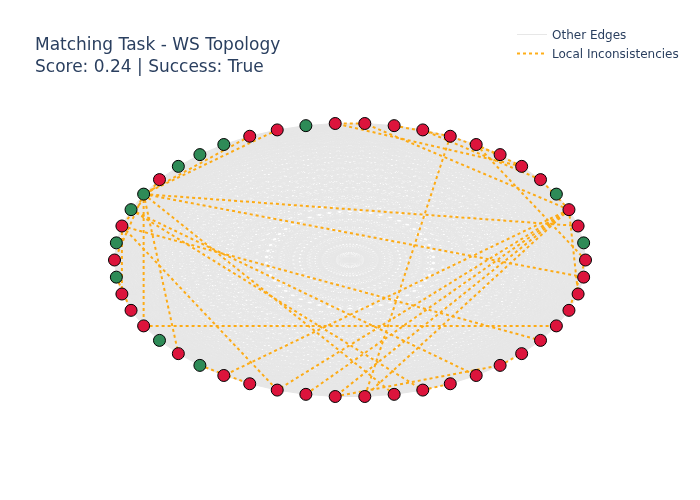
\includegraphics[trim=100 100 90 100,clip,width=0.22\textwidth]{figures/topology/matching_results_20250919_112014_rounds3_gpt-4o-mini_nodes50_concordia_matching_original.png}}
    \subfloat[All ($n=100$)]{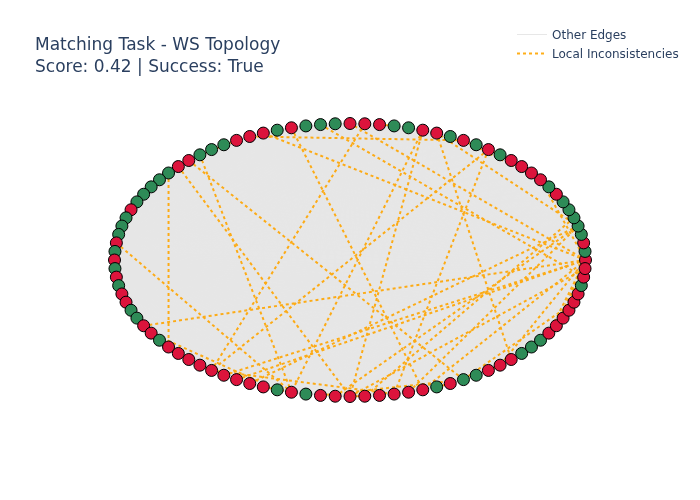
\includegraphics[trim=100 100 90 100,clip,width=0.26\textwidth]{figures/topology/matching_results_20250919_110457_rounds3_gpt-4o-mini_nodes100_concordia_matching_original.png}}
    \\
    \vspace{2mm}
    \caption{Matching experiment outcomes using the \emph{original scoring model}. Each agent selects one of its neighbors (or ``None'') to form a pair. Green nodes denote agents whose selections are locally consistent---that is, they selected a valid neighbor who reciprocated the choice. Red nodes represent agents involved in inconsistencies, such as choosing a non-neighbor, selecting a non-reciprocating partner, or forming idle pairs where both neighbors chose ``None.'' The overall score corresponds to the fraction of locally consistent agents, following the computation described in the text.}


    \label{fig:matching-results}
\end{figure*}

% 
\begin{figure*}[t]
    \centering
    % --- WS ---
    \subfloat[SW ($n=4$)]{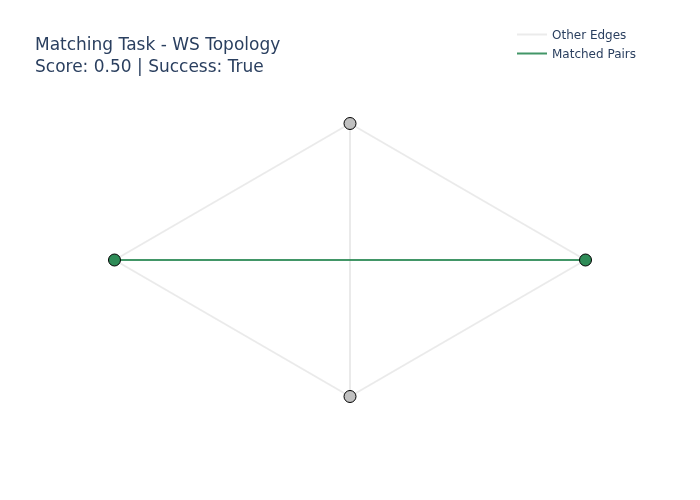
\includegraphics[trim=100 100 90 100,clip,width=0.12\textwidth]{figures/topology/matching_results_20250917_224359_rounds8_gpt-4o-mini_nodes4_langgraph_matching.png}}
    \subfloat[SW ($n=8$)]{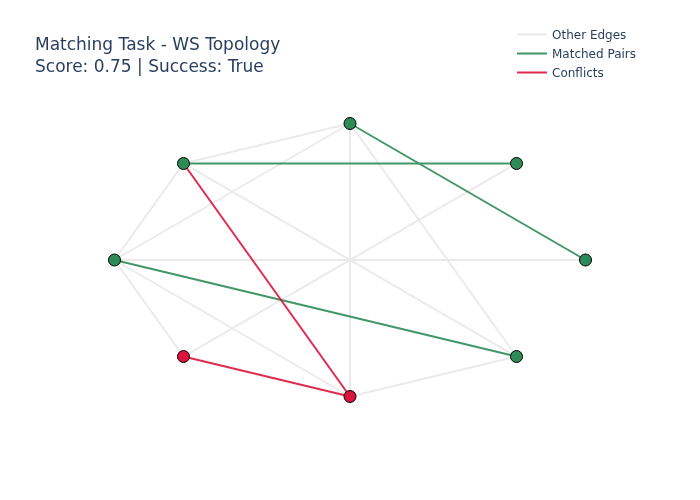
\includegraphics[trim=100 100 90 100,clip,width=0.16\textwidth]{figures/topology/matching_results_20250917_224622_rounds8_gpt-4o-mini_nodes8_langgraph_matching.png}}
    \subfloat[SW ($n=16$)]{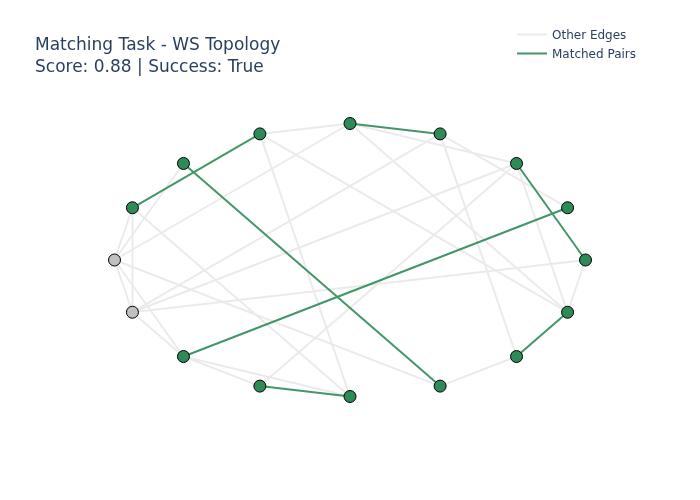
\includegraphics[trim=100 100 90 100,clip,width=0.19\textwidth]{figures/topology/matching_results_20250917_224907_rounds8_gpt-4o-mini_nodes16_langgraph_matching.png}}
    \subfloat[SW ($n=50$)]{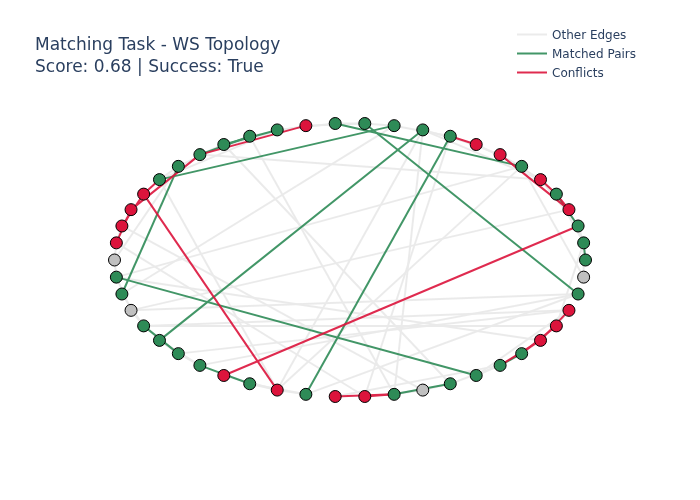
\includegraphics[trim=100 100 90 100,clip,width=0.22\textwidth]{figures/topology/matching_results_20250920_223026_rounds11_gpt-4o-mini_nodes50_langgraph_matching.png}}
    \subfloat[SW ($n=100$)]{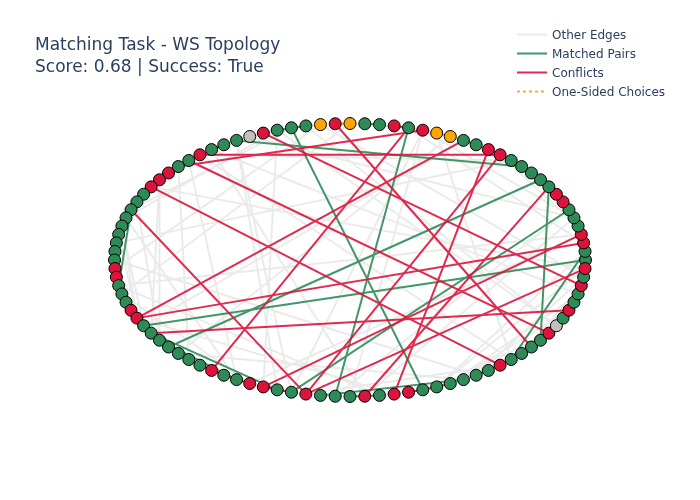
\includegraphics[trim=100 100 90 100,clip,width=0.26\textwidth]{figures/topology/matching_results_20250919_123428_rounds15_gpt-4o-mini_nodes100_langgraph_matching.png}}
    \\
    \vspace{2mm}
    % --- BA ---
    \subfloat[SF ($n=4$)]{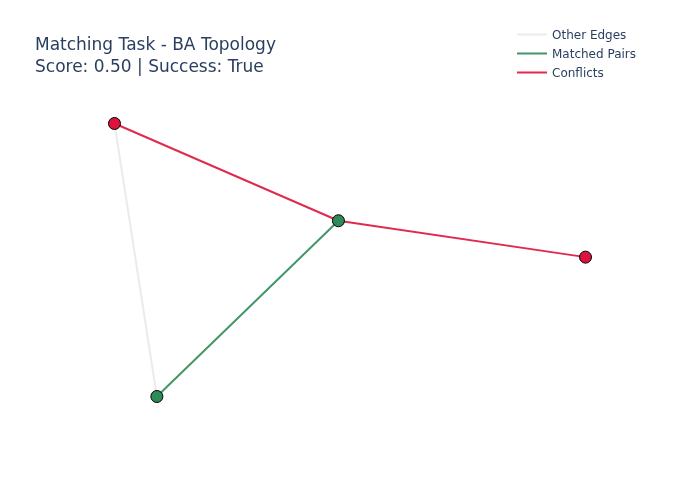
\includegraphics[trim=100 100 90 100,clip,width=0.12\textwidth]{figures/topology/matching_results_20250917_225048_rounds8_gpt-4o-mini_nodes4_langgraph_matching.png}}
    \subfloat[SF ($n=8$)]{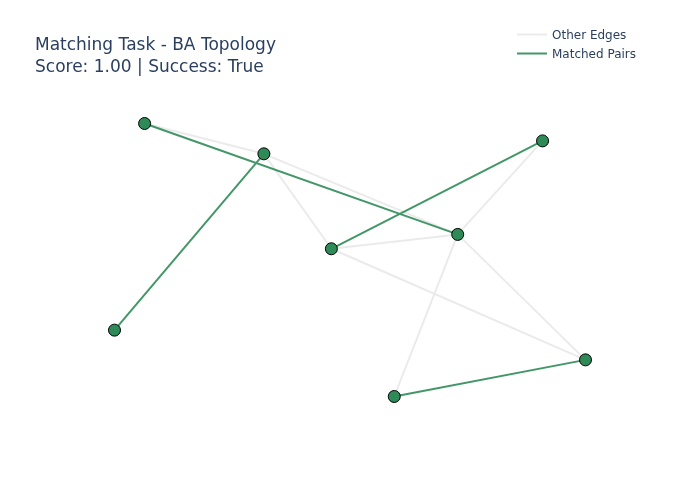
\includegraphics[trim=100 100 90 100,clip,width=0.16\textwidth]{figures/topology/matching_results_20250917_225237_rounds8_gpt-4o-mini_nodes8_langgraph_matching.png}}
    \subfloat[SF ($n=16$)]{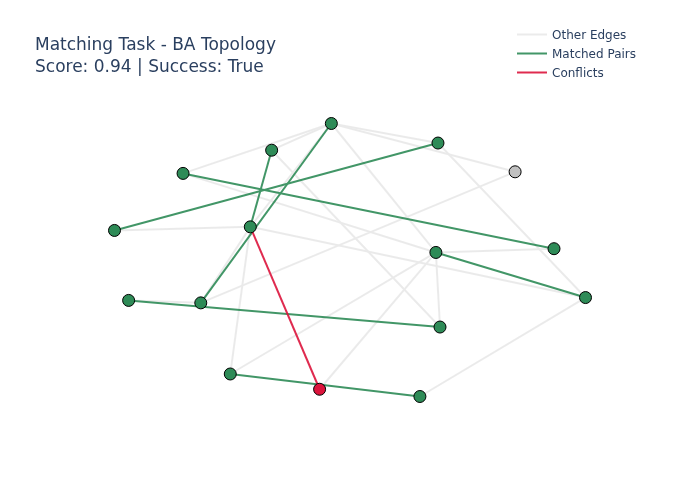
\includegraphics[trim=100 100 90 100,clip,width=0.19\textwidth]{figures/topology/matching_results_20250917_225456_rounds8_gpt-4o-mini_nodes16_langgraph_matching.png}}
    \subfloat[SF ($n=50$)]{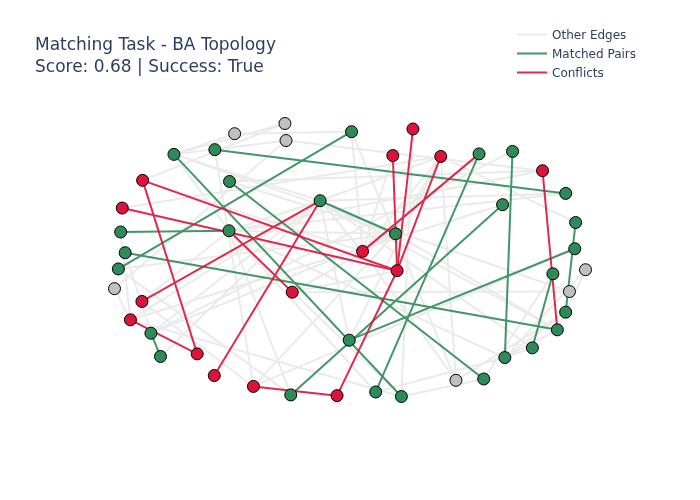
\includegraphics[trim=100 100 90 100,clip,width=0.22\textwidth]{figures/topology/matching_results_20250920_180551_rounds11_gpt-4o-mini_nodes50_langgraph_matching.png}}
    \subfloat[SF ($n=100$)]{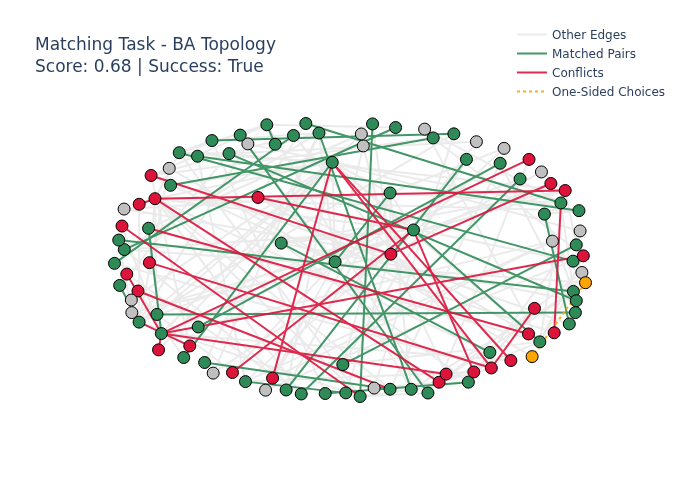
\includegraphics[trim=100 100 90 100,clip,width=0.26\textwidth]{figures/topology/matching_results_20250920_181618_rounds11_gpt-4o-mini_nodes100_langgraph_matching.png}}
    \\
    \vspace{2mm}
    % --- DT ---
    \subfloat[DT ($n=4$)]{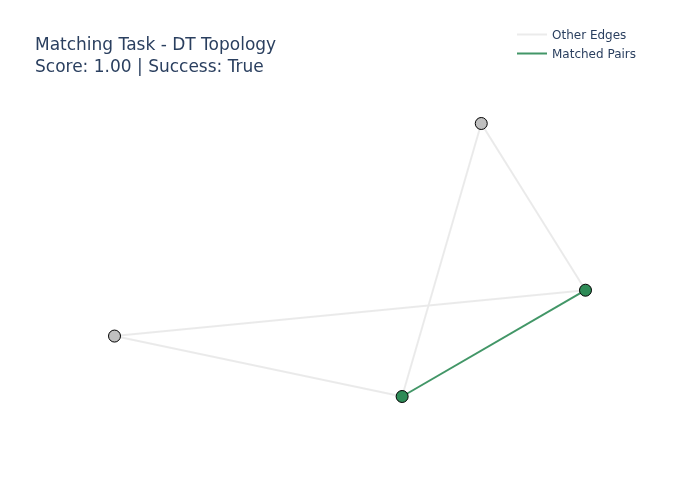
\includegraphics[trim=100 100 90 100,clip,width=0.12\textwidth]{figures/topology/matching_results_20250917_225625_rounds8_gpt-4o-mini_nodes4_langgraph_matching.png}}
    \subfloat[DT ($n=8$)]{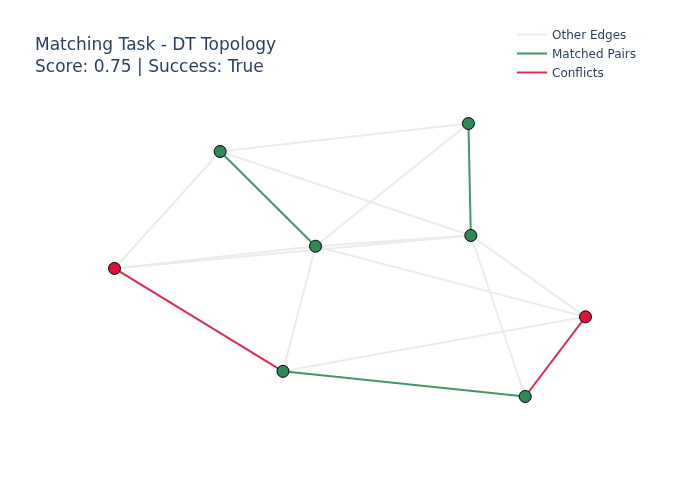
\includegraphics[trim=100 100 90 100,clip,width=0.16\textwidth]{figures/topology/matching_results_20250917_225759_rounds8_gpt-4o-mini_nodes8_langgraph_matching.png}}
    \subfloat[DT ($n=16$)]{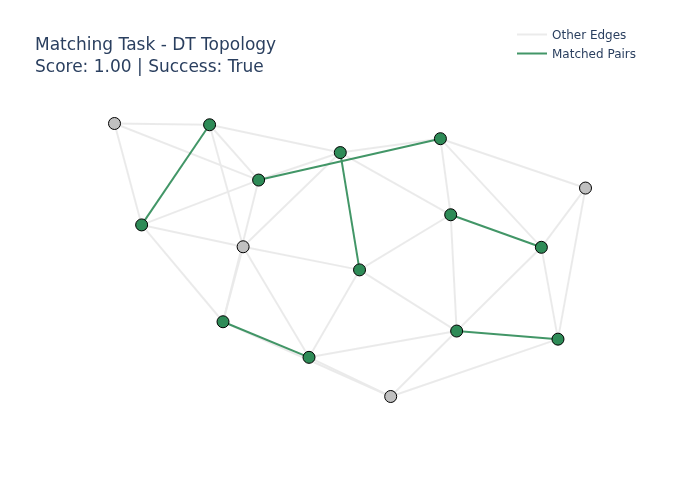
\includegraphics[trim=100 100 90 100,clip,width=0.19\textwidth]{figures/topology/matching_results_20250917_230008_rounds8_gpt-4o-mini_nodes16_langgraph_matching.png}}
    \subfloat[DT ($n=50$)]{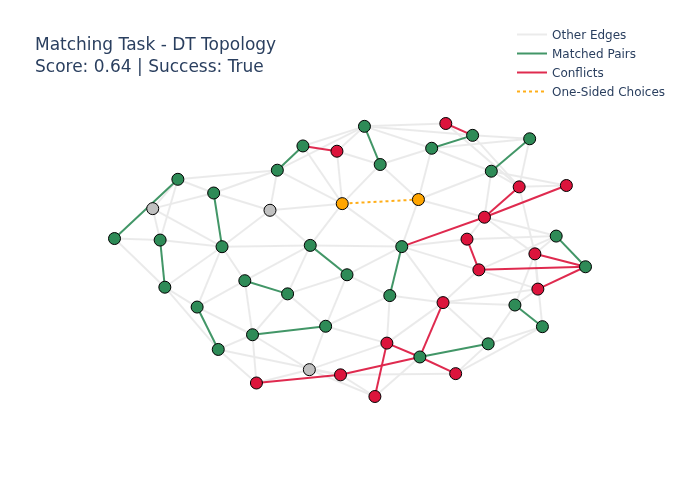
\includegraphics[trim=100 100 90 100,clip,width=0.22\textwidth]{figures/topology/matching_results_20250920_182438_rounds13_gpt-4o-mini_nodes50_langgraph_matching.png}}
    \subfloat[DT ($n=100$)]{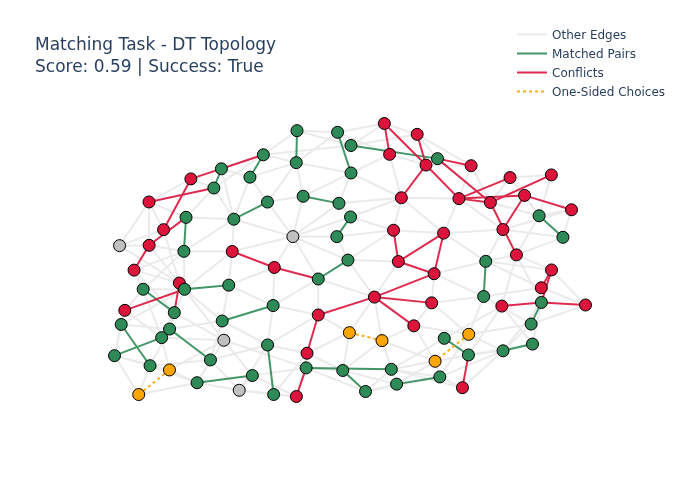
\includegraphics[trim=100 100 90 100,clip,width=0.26\textwidth]{figures/topology/matching_results_20250920_184622_rounds19_gpt-4o-mini_nodes100_langgraph_matching.png}}
    \\
    \vspace{2mm}
    % --- SEQUENTIAL ---
    \subfloat[Seq. ($n=4$)]{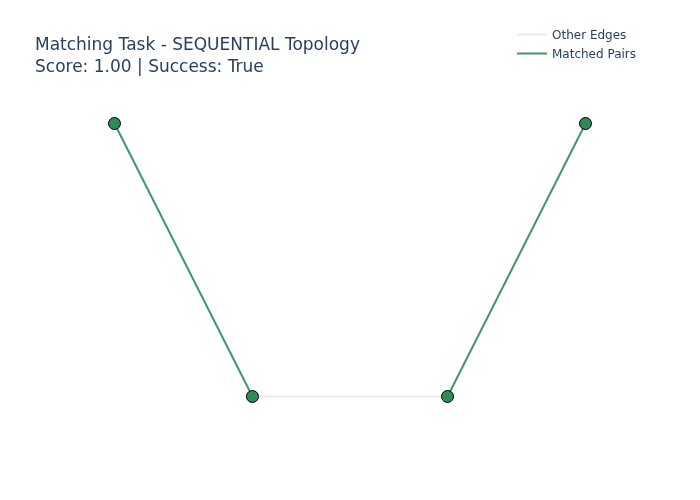
\includegraphics[trim=100 100 90 100,clip,width=0.12\textwidth]{figures/topology/matching_results_20250924_134419_rounds8_gpt-4o-mini_nodes4_crewai-sequential_matching.png}}
    \subfloat[Seq. ($n=8$)]{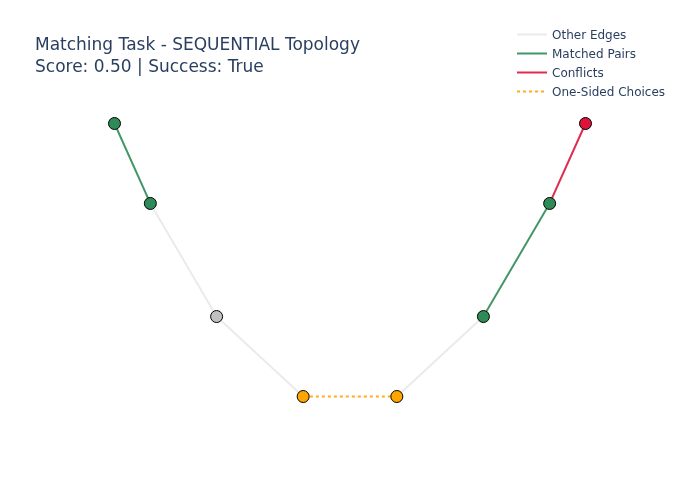
\includegraphics[trim=100 100 90 100,clip,width=0.16\textwidth]{figures/topology/matching_results_20250924_134606_rounds8_gpt-4o-mini_nodes8_crewai-sequential_matching.png}}
    \subfloat[Seq. ($n=16$)]{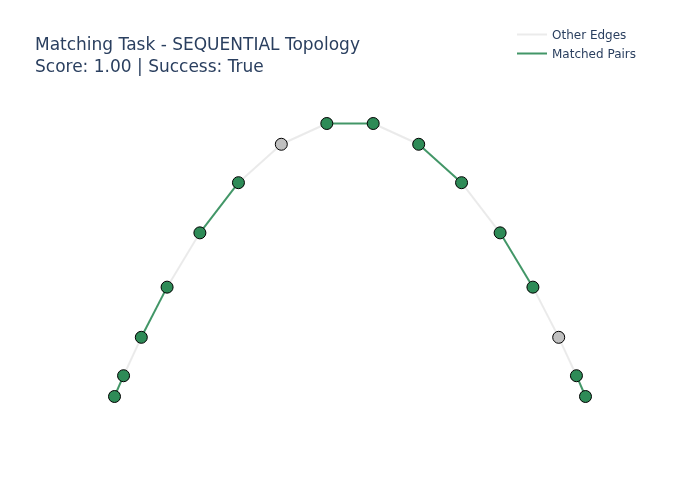
\includegraphics[trim=100 100 90 100,clip,width=0.19\textwidth]{figures/topology/matching_results_20250924_134833_rounds8_gpt-4o-mini_nodes16_crewai-sequential_matching.png}}
    \subfloat{\rule{0.22\textwidth}{0pt}} % placeholder without number
    \subfloat{\rule{0.26\textwidth}{0pt}} % placeholder without number
    \\
    \vspace{2mm}
    % --- HIERARCHICAL ---
    \subfloat[Hier. ($n=4$)]{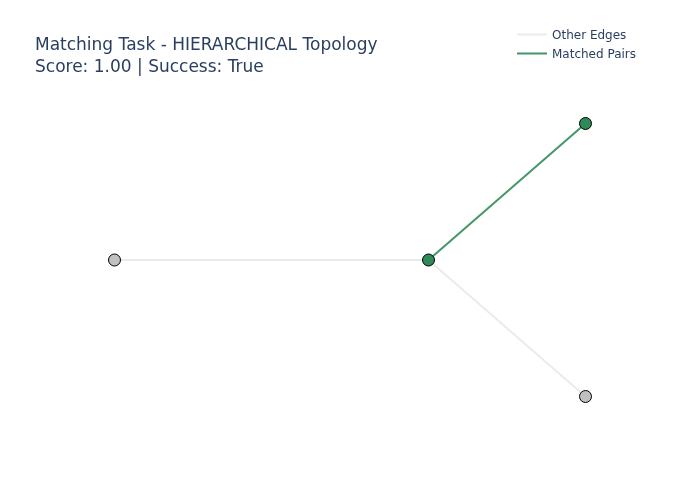
\includegraphics[trim=100 100 90 100,clip,width=0.12\textwidth]{figures/topology/matching_results_20250924_144228_rounds8_gpt-4o-mini_nodes4_crewai-hierarchical_matching.png}}
    \subfloat[Hier. ($n=8$)]{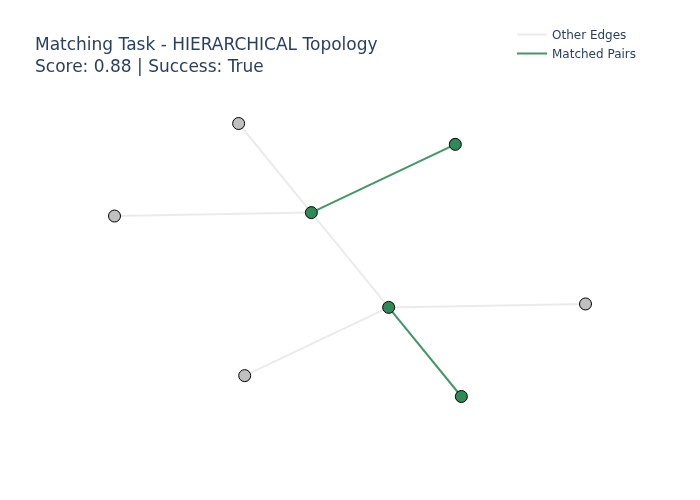
\includegraphics[trim=100 100 90 100,clip,width=0.16\textwidth]{figures/topology/matching_results_20250924_144411_rounds8_gpt-4o-mini_nodes8_crewai-hierarchical_matching.png}}
    \subfloat[Hier. ($n=16$)]{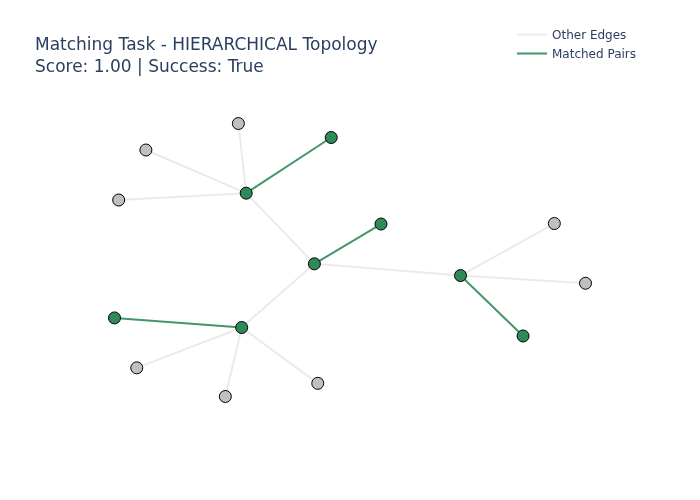
\includegraphics[trim=100 100 90 100,clip,width=0.19\textwidth]{figures/topology/matching_results_20250924_144629_rounds8_gpt-4o-mini_nodes16_crewai-hierarchical_matching.png}}
    \subfloat[Hier. ($n=50$)]{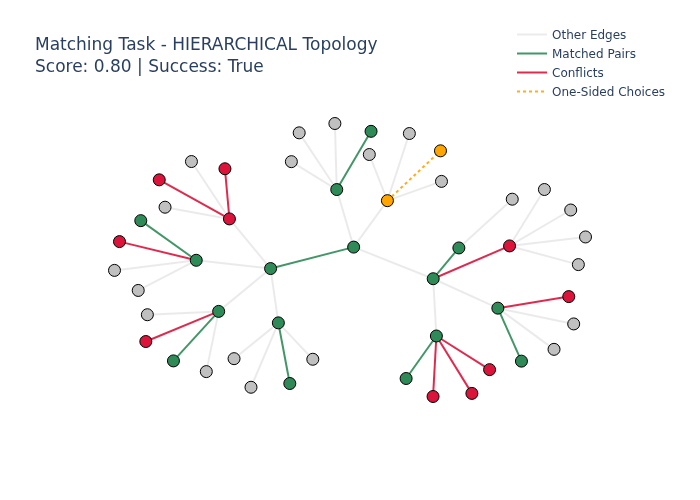
\includegraphics[trim=100 100 90 100,clip,width=0.22\textwidth]{figures/topology/matching_results_20250925_001343_rounds13_gpt-4o-mini_nodes50_crewai-hierarchical_matching.png}}
    \subfloat[Hier. ($n=100$)]{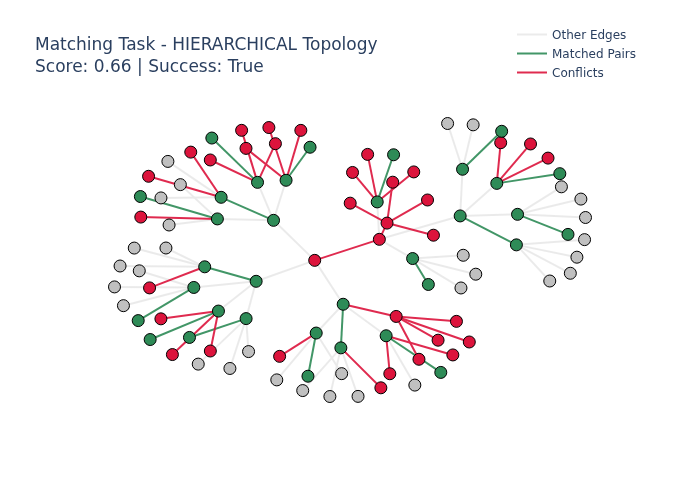
\includegraphics[trim=100 100 90 100,clip,width=0.26\textwidth]{figures/topology/matching_results_20250925_002721_rounds15_gpt-4o-mini_nodes100_crewai-hierarchical_matching.png}}
    \\
    \vspace{2mm}
    % --- ALL ---
    \subfloat[All ($n=4$)]{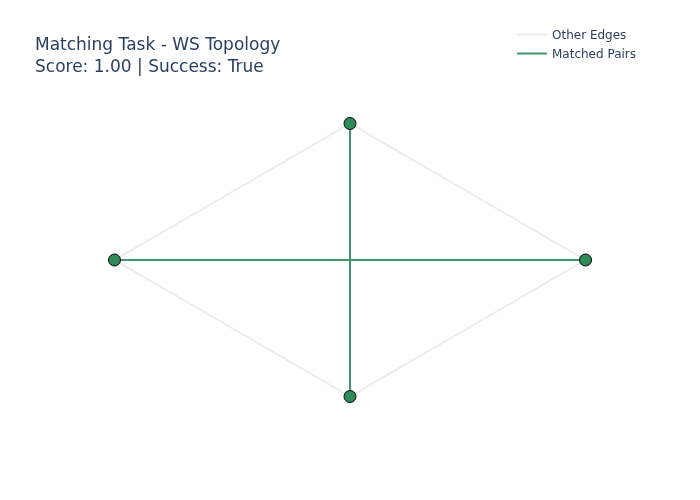
\includegraphics[trim=100 100 90 100,clip,width=0.12\textwidth]{figures/topology/matching_results_20250917_230141_rounds8_gpt-4o-mini_nodes4_concordia_matching.png}}
    \subfloat[All ($n=8$)]{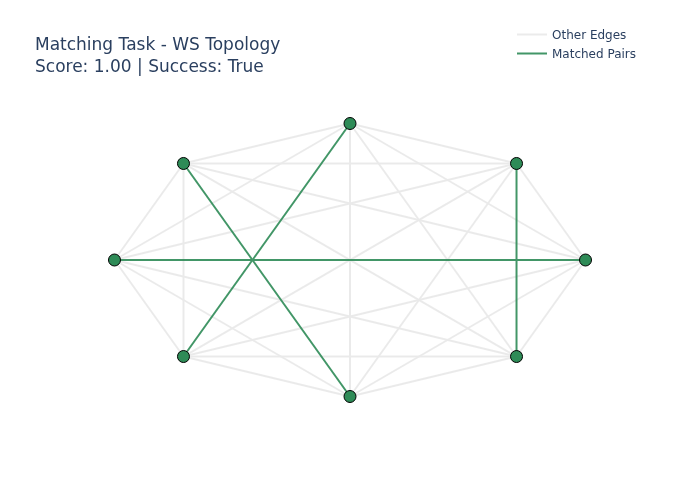
\includegraphics[trim=100 100 90 100,clip,width=0.16\textwidth]{figures/topology/matching_results_20250917_230411_rounds8_gpt-4o-mini_nodes8_concordia_matching.png}}
    \subfloat[All ($n=16$)]{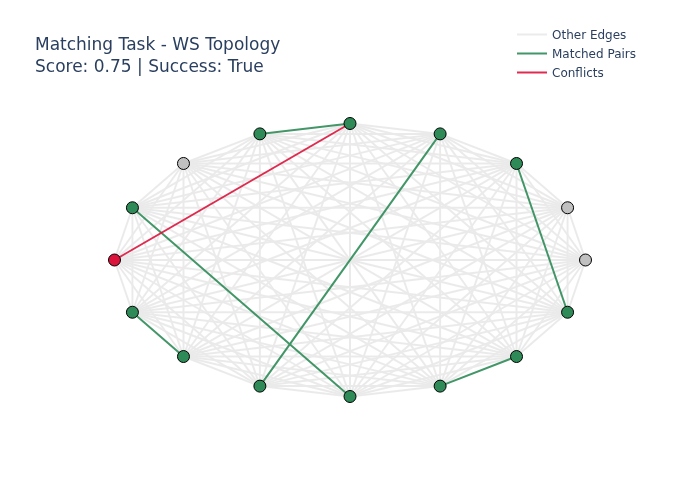
\includegraphics[trim=100 100 90 100,clip,width=0.19\textwidth]{figures/topology/matching_results_20250917_230756_rounds8_gpt-4o-mini_nodes16_concordia_matching.png}}
    \subfloat[All ($n=50$)]{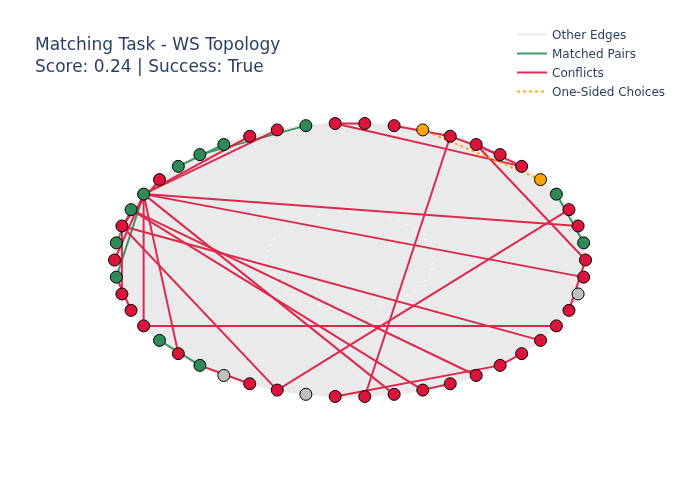
\includegraphics[trim=100 100 90 100,clip,width=0.22\textwidth]{figures/topology/matching_results_20250919_112014_rounds3_gpt-4o-mini_nodes50_concordia_matching.png}}
    \subfloat[All ($n=100$)]{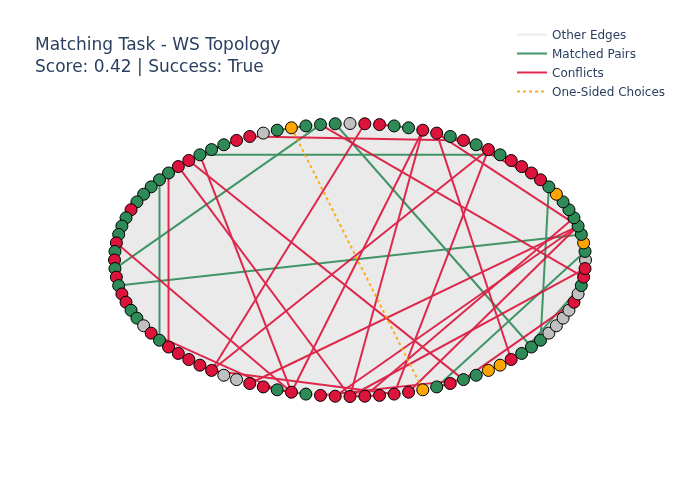
\includegraphics[trim=100 100 90 100,clip,width=0.26\textwidth]{figures/topology/matching_results_20250919_110457_rounds3_gpt-4o-mini_nodes100_concordia_matching.png}}
    \\
    \vspace{2mm}
    \caption{Matching experiment outcomes across different network sizes ($n=4$ to $100$). Each subfigure shows the final pair assignments of agents based on the enhanced local-consistency model. Green edges connect mutually consistent agents whose choices satisfy the neighbor-reciprocation rule; orange dotted edges denote one-sided or invalid selections; and red nodes highlight agents involved in any local inconsistency. Gray edges represent structural links that did not participate in the matching process. This visualization extends the local scoring logic to explicitly reveal consistent and conflicting interactions.}

    \label{fig:matching-results-modified}
\end{figure*}


% \input{figures/topology_latex/leader}
% \input{figures/topology_latex/vertex}















\newpage

\section{Extended Topology Scalability Details and Visual Results}
\label{appendix:extended}

This appendix provides extended methodological details and full visualization results supporting the coordination and scalability experiments reported in Section~\ref{sec:Coordination_section}. While the main paper focuses on outcome-level comparisons and cross-task insights, the appendix elaborates on convergence mechanics, topology-dependent failure modes, and agent-level negotiation dynamics. All benchmark definitions and evaluation settings are specified in Section~\ref{subsec:bench_coordination}; the material here complements those sections by exposing how observed behaviors emerge in practice.

\subsection{Experimental Structure and Controls}

All experiments use a fixed LLM configuration, unified prompt template, and shared termination criteria across all runs. Agent initialization, task semantics, and communication rules are held constant so that observed differences reflect only communication topology and orchestration structure. Scalability is evaluated at network sizes
\(n \in \{4, 8, 16, 50, 100\}\), allowing analysis of both small-network reasoning behavior and large-scale coordination breakdown.

For every run, we record success outcome, rounds to convergence, total token consumption, and wall-clock runtime. These metrics are reported in Table~\ref{tab:scalability-results} and analyzed in Section~\ref{sec:Coordination_section}. The appendix focuses on explaining the qualitative mechanisms behind those numeric trends.

\subsection{Rounds-to-Convergence Policy}
\label{appendix:rounds}

AGENTSNET enforces a minimum interaction budget of eight rounds to ensure sufficient message exchange even for small or sparse topologies. Consequently, some runs converge in fewer than eight effective rounds but are still executed under the minimum budget. For global agreement tasks (\textsc{Consensus} and \textsc{LeaderElection}) and for settings with \(n > 16\), the maximum horizon is instead determined by the network diameter \(D\), using
\[
T = 2D + 1,
\]
which guarantees complete information propagation under synchronous message passing. Under this policy, large-scale runs may require between fifteen and nineteen rounds depending on topology diameter. This rule explains why convergence rounds do not monotonically increase with \(n\) and why some large networks converge faster than smaller ones when topology permits early stabilization.

\subsection{Task-Specific Scoring and Visual Encoding}
\label{appendix:scoring}

We adopt the AGENTSNET benchmark~\cite{coordinationcollaborativereasoning} for the task definitions and evaluation criteria. With the exception of \textsc{Matching}, all tasks are evaluated using binary success criteria, reflecting whether the distributed constraint is globally satisfied at termination. Only \textsc{Matching} admits a graded notion of partial correctness by design.

\paragraph{Matching (Maximal Matching).}
In the \textsc{Matching} task, agents attempt to form pairwise agreements with neighboring agents. A match is considered valid if agent \(u\) selects agent \(v\) and agent \(v\) selects agent \(u\). Inconsistencies arise when selections are non-reciprocal, invalid (non-neighbor), or when two adjacent agents both select \texttt{None} despite being able to form a pair. Let \(I\) denote the number of inconsistent agents. Following AGENTSNET, the final score is computed as
\[
\text{Score} = 1 - \frac{I}{|V|}.
\]
This formulation yields a continuous score in \([0,1]\), capturing partial correctness even when a globally maximal matching is not achieved. Visualizations encode reciprocal matches in green, one-sided selections in orange, inconsistent agents in red, and unused edges in gray.

\paragraph{Consensus.}
In the \textsc{Consensus} task, each agent selects a binary value from \(\{0,1\}\). The task is successful if and only if all agents output the same value at termination. Formally, letting \(A(u)\) denote the output of agent \(u\), success is defined as
\[
\exists b \in \{0,1\} \;\; \text{s.t.} \;\; \forall u \in V,\; A(u) = b.
\]
The score is therefore binary. Visualizations depict agent states and communication links, where green links indicate agreement between neighboring agents and red links indicate disagreement.

\paragraph{Coloring (\((\Delta+1)\)-Coloring).}
In the \textsc{Coloring} task, each agent selects a color from a predefined palette of size \(\Delta + 1\), where \(\Delta\) is the maximum node degree. A run is successful if the resulting assignment constitutes a valid coloring, i.e.,
\[
\forall (u,v) \in E,\; \text{color}(u) \neq \text{color}(v).
\]
Success is binary. Visualizations highlight conflict-free edges in green and color collisions in red, revealing how conflicts cluster under different communication structures.

\paragraph{LeaderElection.}
In the \textsc{LeaderElection} task, agents must collectively designate exactly one leader. Each agent outputs either \texttt{Yes} (leader) or \texttt{No} (follower). Let \(A(u)\) denote the response of agent \(u\). A run is successful if
\[
\sum_{u \in V} \mathbf{1}[A(u) = \texttt{Yes}] = 1.
\]
This task is evaluated using a binary success criterion. Visualizations mark the elected leader in green, competing leaders in red, and followers in gray, exposing symmetry-breaking failures.

\paragraph{VertexCover (Minimal Vertex Cover).}
In the \textsc{VertexCover} task, agents decide whether they are members of a coordinating set. Let \(C \subseteq V\) denote the set of agents selecting \texttt{Yes}. A run is successful if \(C\) forms a valid vertex cover, i.e.,
\[
\forall (u,v) \in E,\; u \in C \;\text{or}\; v \in C.
\]
Following AGENTSNET, minimality is assessed qualitatively through visual inspection rather than through a graded score; quantitative evaluation reports binary success. Visualizations distinguish minimal cover nodes (green), non-minimal but valid selections (blue), invalid responses (orange), and uncovered edges (red).



\subsection{Visualization-Driven Interpretation}
\label{appendix:visualization}

Figures in this appendix present complete visual outputs for all tasks, topologies, and network sizes, revealing how coordination succeeds or fails at the agent level.

\paragraph{Consensus (Figure~\ref{fig:consensus-results}).}
Fully connected communication maintains unified agreement across all scales, with all agents converging to a single value and no persistent disagreement links even at \(n=100\). Small-world and scale-free topologies preserve partial coherence at small and mid-scale, where agreement clusters remain connected through shortcut edges or hubs, but increasingly fragment as \(n\) grows. At large scale, disagreement links form stable boundaries between local clusters, explaining why these topologies incur high communication cost without achieving full success. Delaunay graphs exhibit the strongest fragmentation: agreement remains confined to small geometric neighborhoods, and isolated disagreement clusters persist even after the maximum round budget, directly corresponding to the systematic failure trends observed in Table~\ref{tab:scalability-results}.

\paragraph{Coloring (Figure~\ref{fig:coloring-results}).}
Scale-free and small-world topologies maintain stable chromatic separation across scales, with conflicts resolved early and remaining localized even as the network grows. The visualizations show that hub-mediated diffusion in scale-free graphs allows color constraints to propagate efficiently, preventing large-scale cascades of conflicts. In contrast, Delaunay graphs increasingly exhibit localized conflict regions at higher \(n\), where geometric isolation delays conflict resolution and produces persistent red edges, consistent with the higher convergence cost and reduced stability reported in the quantitative results.

\paragraph{Matching (Figures~\ref{fig:matching-results}–\ref{fig:matching-results-modified}).}
Diffusion-friendly topologies preserve reciprocal agreement at moderate scale, with most matches forming clean, mutually consistent pairs. As network size increases, small-world and scale-free graphs begin to show isolated pockets of one-sided selections, but these remain relatively sparse. In contrast, geometric Delaunay graphs degrade sharply: one-sided selections and inconsistent agents proliferate across the network, forming dense regions of orange and red nodes. These visual patterns explain why Matching success declines and token cost increases substantially for geometric topologies, even when rounds are allowed to scale.

\paragraph{LeaderElection (Figure~\ref{fig:leader-results}).}
LeaderElection exhibits a distinct visual regime. Diffusion-based topologies consistently generate multiple competing leader candidates that persist across rounds, forming stable red clusters that are not resolved by increased communication. Geometric locality, while costly, enables eventual suppression of competing leaders, producing a single green leader at larger scales after extended coordination. Hierarchical orchestration further accelerates symmetry breaking at small and medium scales, but visualizations reveal increasing instability at large \(n\), where depth-induced delays allow competing leader branches to emerge, aligning with the degradation observed in the table.

\paragraph{VertexCover (Figure~\ref{fig:vertexcover-results}).}
Small-world and scale-free topologies converge toward compact vertex covers, with most edges covered by a small set of coordinating nodes and limited over-selection. As scale increases, these topologies maintain relatively structured cover patterns, explaining their higher success despite moderate communication cost. In contrast, Delaunay and hierarchical structures frequently over-cover, selecting excessive coordinating nodes, or leave uncovered edges at large \(n\). The visualizations reveal that geometric locality and hierarchical bottlenecks prevent agents from globally coordinating coverage decisions, leading to inefficiencies and constraint violations consistent with the quantitative breakdown.

% \subsection{Cross-Task Scalability Summary}
% \label{appendix:summary}

% Across tasks and scales, three consistent patterns emerge. First, topologies that support fast information diffusion—such as small-world and scale-free graphs—are better suited for negotiation and conflict resolution tasks, sustaining partial correctness even under increasing load. Second, structured orchestration mechanisms facilitate symmetry-breaking tasks like \textsc{LeaderElection} but become brittle as coordination depth grows. Third, centralized broadcast communication reliably enforces global agreement but incurs rapidly increasing communication cost as scale increases. Together, the visual evidence complements the quantitative results by revealing how communication geometry shapes not only whether coordination succeeds, but how failure modes emerge and persist as multi-agent systems scale.


\begin{figure*}[t]
    \centering
    % --- Row 1 ---
    \subfloat[SW ($n=4$)]{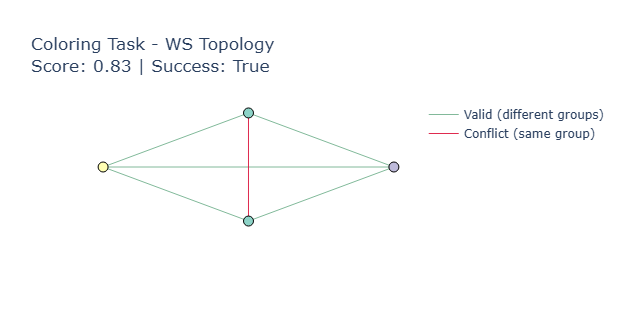
\includegraphics[trim=90 80 200 100,clip,width=0.12\textwidth]{figures/topology/coloring_results_20250917_222432_rounds8_gpt-4o-mini_nodes4.png}}
    \subfloat[SW ($n=8$)]{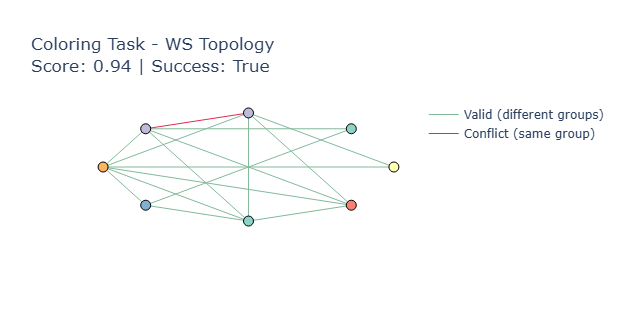
\includegraphics[trim=90 80 200 100,clip,width=0.16\textwidth]{figures/topology/coloring_results_20250917_222635_rounds8_gpt-4o-mini_nodes8.png}}
    \subfloat[SW ($n=16$)]{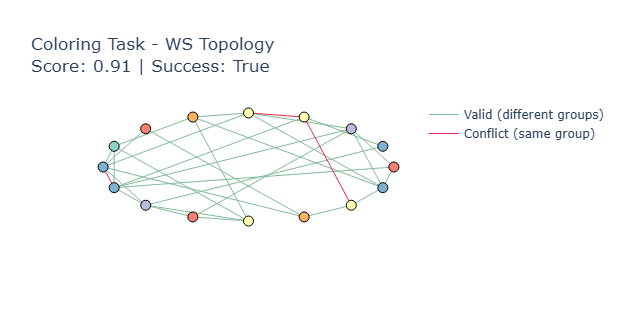
\includegraphics[trim=90 80 200 100,clip,width=0.19\textwidth]{figures/topology/coloring_results_20250917_222842_rounds8_gpt-4o-mini_nodes16.png}}
    \subfloat[SW ($n=50$)]{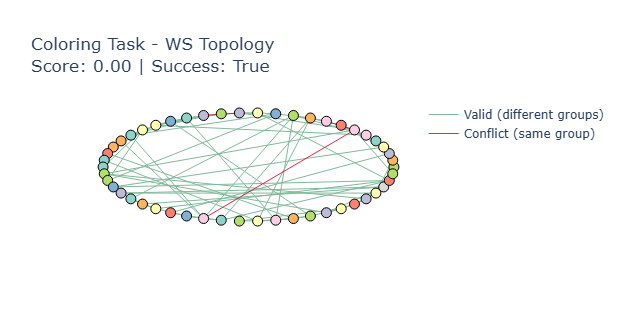
\includegraphics[trim=90 80 200 100,clip,width=0.22\textwidth]{figures/topology/coloring_results_20250920_135347_rounds11_gpt-4o-mini_nodes50.png}}
    \subfloat[SW ($n=100$)]{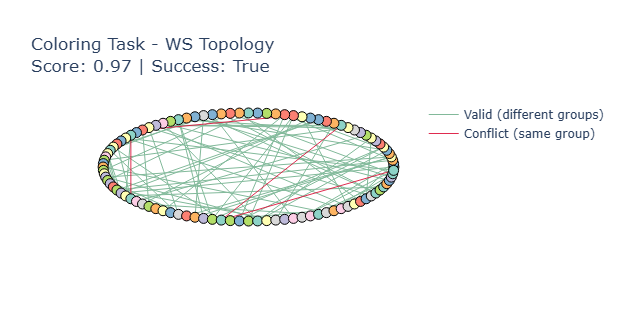
\includegraphics[trim=90 80 200 100,clip,width=0.26\textwidth]{figures/topology/coloring_results_20250920_141018_rounds15_gpt-4o-mini_nodes100.png}}

    % --- Row 2 ---
    \subfloat[SF ($n=4$)]{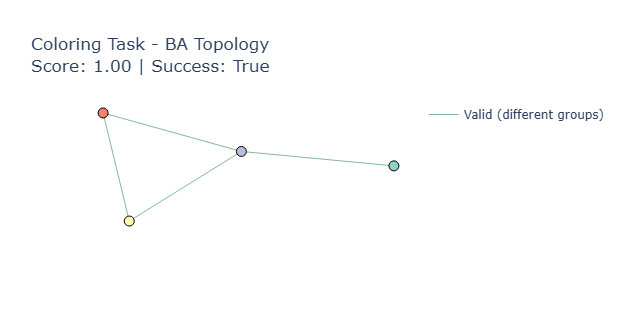
\includegraphics[trim=90 80 200 100,clip,width=0.12\textwidth]{figures/topology/coloring_results_20250917_223003_rounds8_gpt-4o-mini_nodes4.png}}
    \subfloat[SF ($n=8$)]{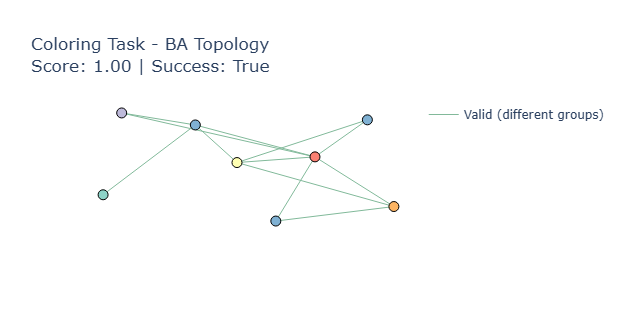
\includegraphics[trim=90 80 200 100,clip,width=0.16\textwidth]{figures/topology/coloring_results_20250917_223205_rounds8_gpt-4o-mini_nodes8.png}} 
    \subfloat[SF ($n=16$)]{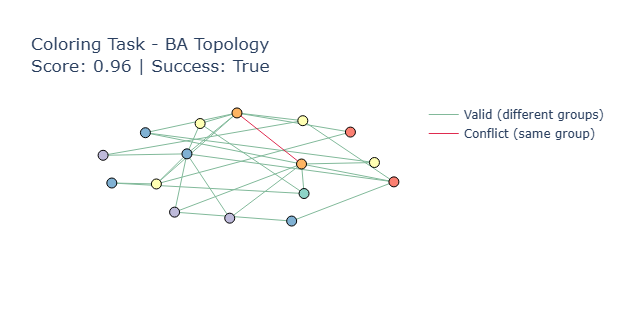
\includegraphics[trim=90 80 200 100,clip,width=0.19\textwidth]{figures/topology/coloring_results_20250917_223421_rounds8_gpt-4o-mini_nodes16.png}}
    \subfloat[SF ($n=50$)]{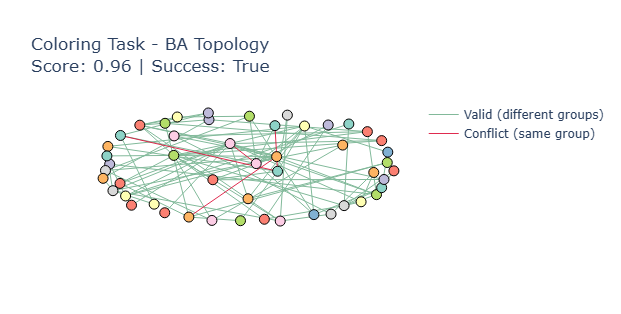
\includegraphics[trim=90 80 200 100,clip,width=0.22\textwidth]{figures/topology/coloring_results_20250920_141717_rounds11_gpt-4o-mini_nodes50.png}}
    \subfloat[SF ($n=100$)]{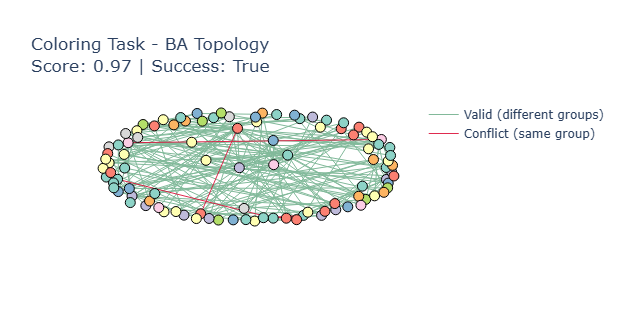
\includegraphics[trim=90 80 200 100,clip,width=0.26\textwidth]{figures/topology/coloring_results_20250920_142903_rounds11_gpt-4o-mini_nodes100.png}}

    % --- Row 3 ---
    \subfloat[DT ($n=4$)]{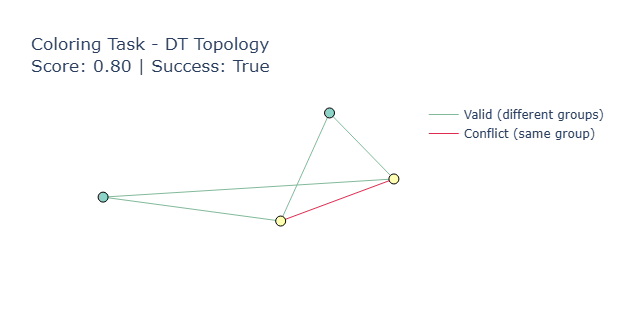
\includegraphics[trim=90 80 200 100,clip,width=0.12\textwidth]{figures/topology/coloring_results_20250917_223636_rounds8_gpt-4o-mini_nodes4.png}}
    \subfloat[DT ($n=8$)]{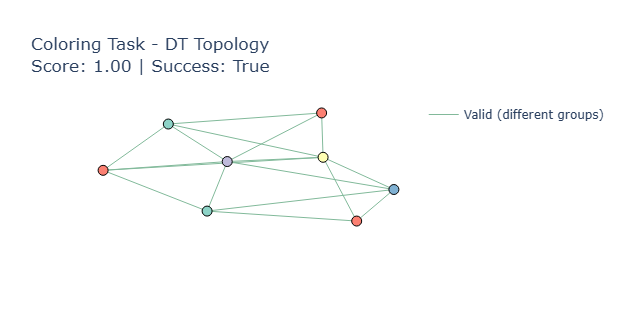
\includegraphics[trim=90 80 200 100,clip,width=0.16\textwidth]{figures/topology/coloring_results_20250917_223854_rounds8_gpt-4o-mini_nodes8.png}}
    \subfloat[DT ($n=16$)]{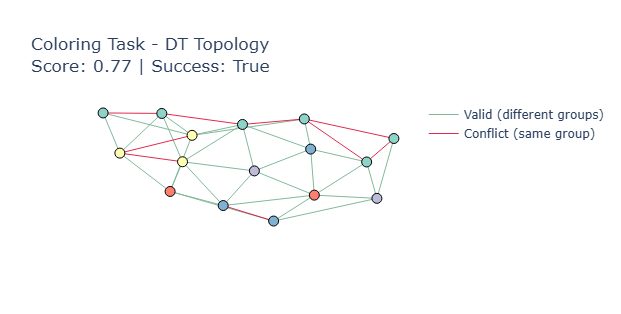
\includegraphics[trim=90 80 200 100,clip,width=0.19\textwidth]{figures/topology/coloring_results_20250917_224151_rounds8_gpt-4o-mini_nodes16.png}} 
    \subfloat[DT ($n=50$)]{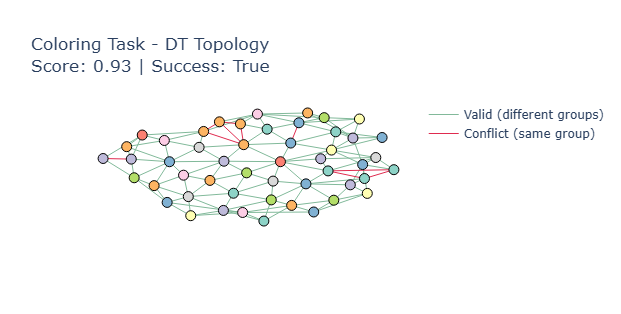
\includegraphics[trim=90 80 200 100,clip,width=0.22\textwidth]{figures/topology/coloring_results_20250920_143802_rounds13_gpt-4o-mini_nodes50.png}} 
    \subfloat[DT ($n=100$)]{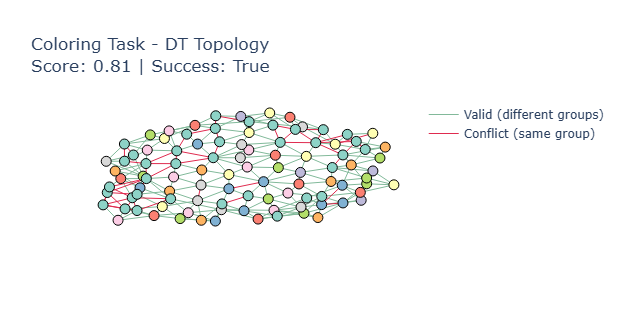
\includegraphics[trim=90 80 200 100,clip,width=0.26\textwidth]{figures/topology/coloring_results_20250920_145919_rounds19_gpt-4o-mini_nodes100.png}} \\



    \vspace{2mm}
    % --- Row 4 ---
    \subfloat[Seq. ($n=4$)]{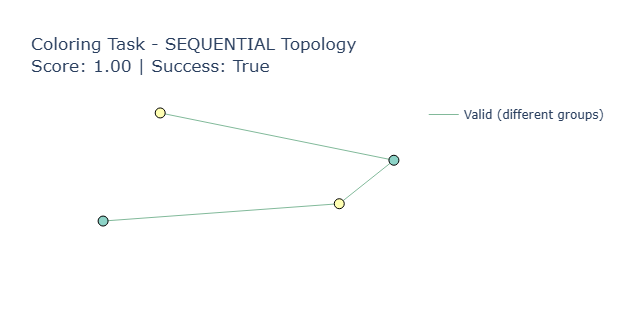
\includegraphics[trim=90 80 200 100,clip,width=0.12\textwidth]{figures/topology/coloring_results_20250924_130551_rounds8_gpt-4o-mini_nodes4.png}}
    \subfloat[Seq. ($n=8$)]{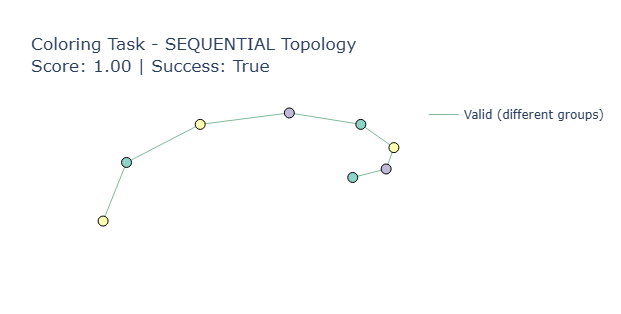
\includegraphics[trim=90 80 200 100,clip,width=0.16\textwidth]{figures/topology/coloring_results_20250924_130747_rounds8_gpt-4o-mini_nodes8.png}}
    \subfloat[Seq. ($n=16$)]{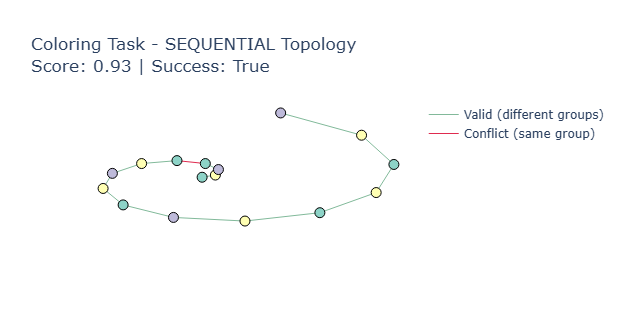
\includegraphics[trim=90 80 200 100,clip,width=0.19\textwidth]{figures/topology/coloring_results_20250924_131004_rounds8_gpt-4o-mini_nodes16.png}} 
    \subfloat{\rule{0.22\textwidth}{0pt}} % placeholder without number
    \subfloat{\rule{0.26\textwidth}{0pt}} % placeholder without number



    % --- Row 5 ---
    \subfloat[Hier. ($n=4$)]{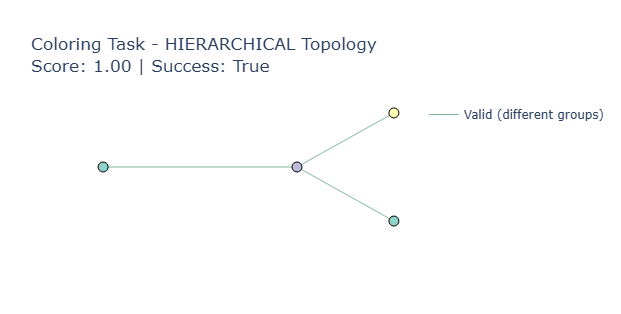
\includegraphics[trim=90 80 200 100,clip,width=0.12\textwidth]{figures/topology/coloring_results_20250924_143605_rounds8_gpt-4o-mini_nodes4.png}}
    \subfloat[Hier. ($n=8$)]{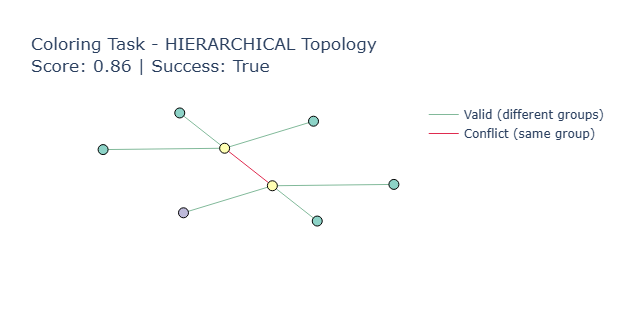
\includegraphics[trim=90 80 200 100,clip,width=0.16\textwidth]{figures/topology/coloring_results_20250924_143802_rounds8_gpt-4o-mini_nodes8.png}}
    \subfloat[Hier. ($n=16$)]{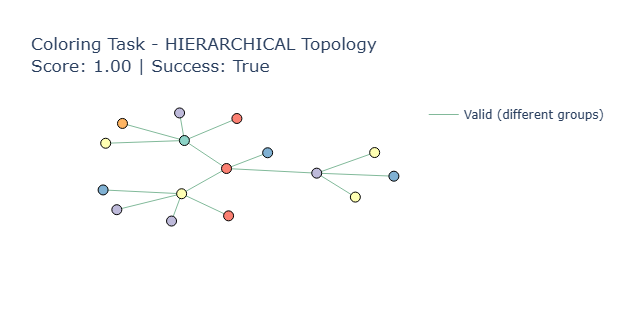
\includegraphics[trim=90 80 200 100,clip,width=0.19\textwidth]{figures/topology/coloring_results_20250924_144052_rounds8_gpt-4o-mini_nodes16.png}} 
    \subfloat[Hier. ($n=50$)]{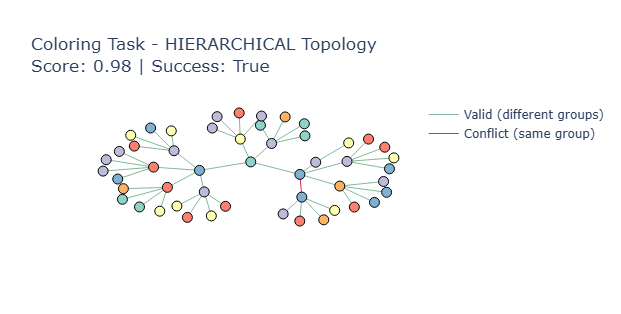
\includegraphics[trim=90 80 200 100,clip,width=0.22\textwidth]{figures/topology/coloring_results_20250924_235040_rounds13_gpt-4o-mini_nodes50}} 
    \subfloat[Hier. ($n=100$)]{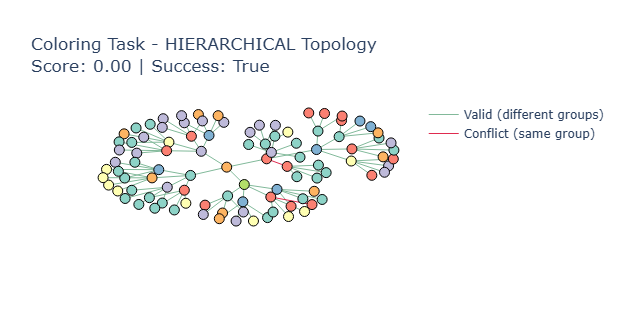
\includegraphics[trim=90 80 200 100,clip,width=0.26\textwidth]{figures/topology/coloring_results_20250925_000609_rounds15_gpt-4o-mini_nodes100}} \\

    \caption{Coloring experiment outcomes across different network sizes ($n=4$ to $100$). 
    Each subfigure shows the final group assignments of agents. 
    Valid assignments (neighbors in different groups) are shown in green, while conflicts (neighbors in the same group) are shown in red.}
    \label{fig:coloring-results}
\end{figure*}

\begin{figure*}[t]
    \centering
    % --- WS ---
    \subfloat[SW ($n=4$)]{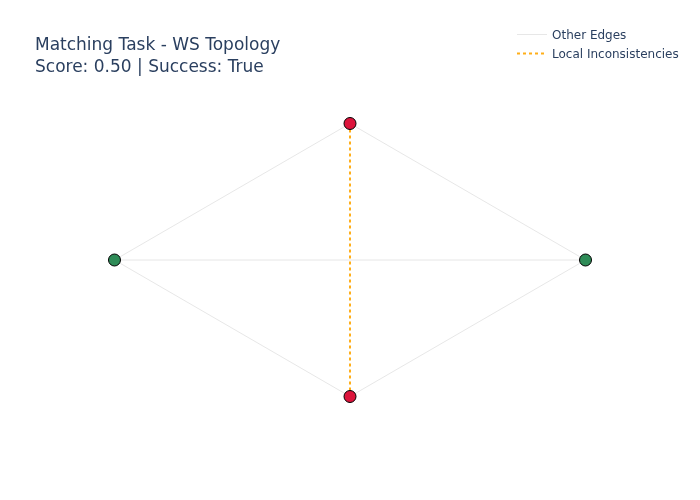
\includegraphics[trim=100 100 90 100,clip,width=0.12\textwidth]{figures/topology/matching_results_20250917_224359_rounds8_gpt-4o-mini_nodes4_langgraph_matching_original.png}}
    \subfloat[SW ($n=8$)]{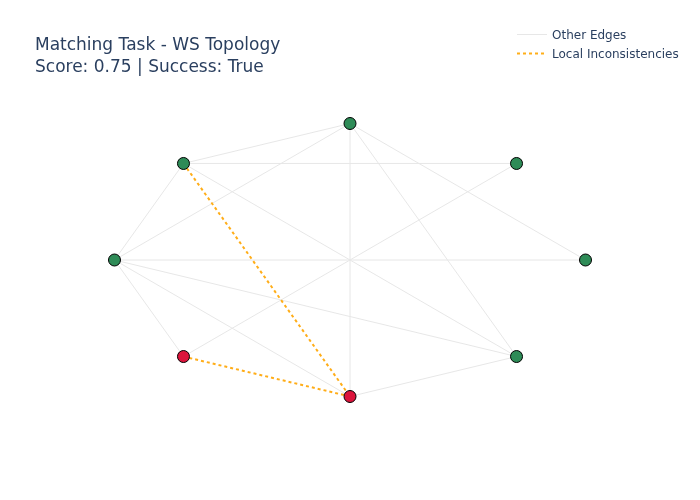
\includegraphics[trim=100 100 90 100,clip,width=0.16\textwidth]{figures/topology/matching_results_20250917_224622_rounds8_gpt-4o-mini_nodes8_langgraph_matching_original.png}}
    \subfloat[SW ($n=16$)]{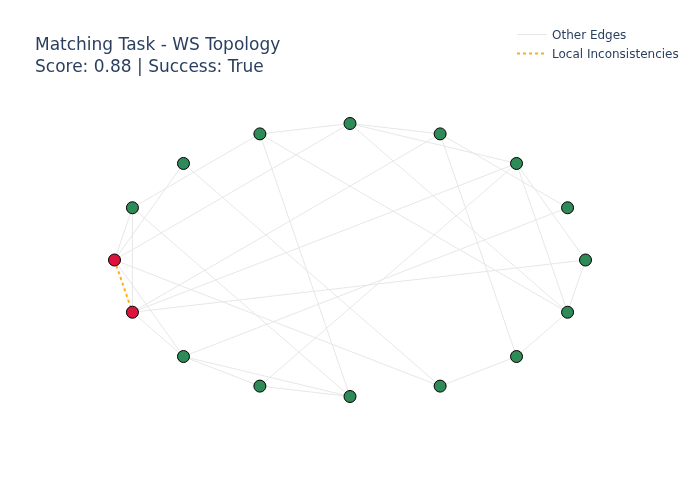
\includegraphics[trim=100 100 90 100,clip,width=0.19\textwidth]{figures/topology/matching_results_20250917_224907_rounds8_gpt-4o-mini_nodes16_langgraph_matching_original.png}}
    \subfloat[SW ($n=50$)]{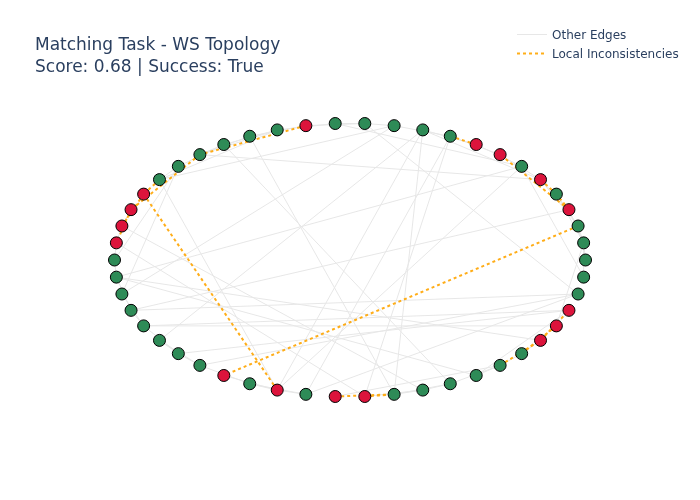
\includegraphics[trim=100 100 90 100,clip,width=0.22\textwidth]{figures/topology/matching_results_20250920_223026_rounds11_gpt-4o-mini_nodes50_langgraph_matching_original.png}}
    \subfloat[SW ($n=100$)]{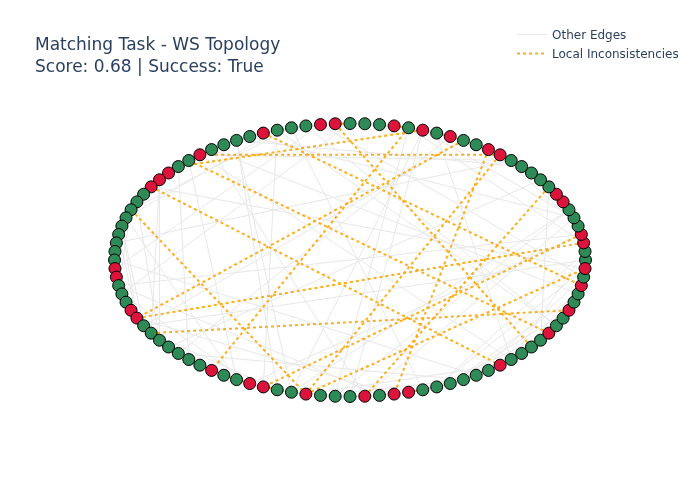
\includegraphics[trim=100 100 90 100,clip,width=0.26\textwidth]{figures/topology/matching_results_20250919_123428_rounds15_gpt-4o-mini_nodes100_langgraph_matching_original.png}}
    \\
    \vspace{2mm}
    % --- BA ---
    \subfloat[SF ($n=4$)]{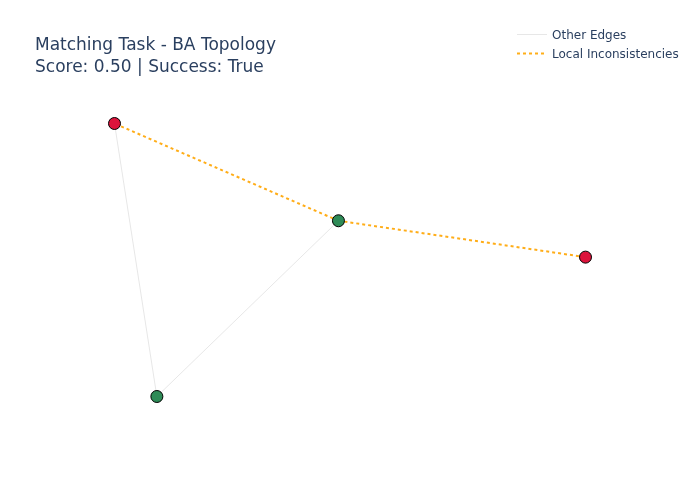
\includegraphics[trim=100 100 90 100,clip,width=0.12\textwidth]{figures/topology/matching_results_20250917_225048_rounds8_gpt-4o-mini_nodes4_langgraph_matching_original.png}}
    \subfloat[SF ($n=8$)]{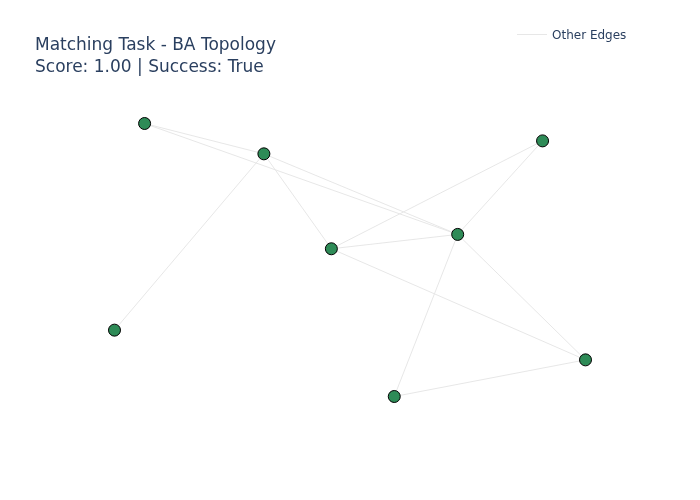
\includegraphics[trim=100 100 90 100,clip,width=0.16\textwidth]{figures/topology/matching_results_20250917_225237_rounds8_gpt-4o-mini_nodes8_langgraph_matching_original.png}}
    \subfloat[SF ($n=16$)]{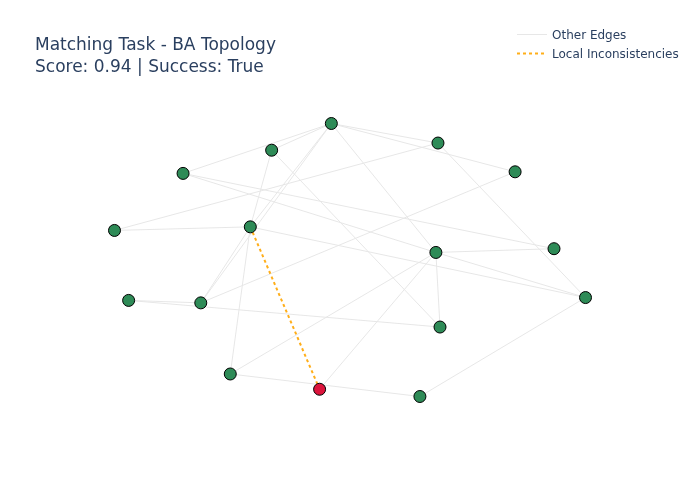
\includegraphics[trim=100 100 90 100,clip,width=0.19\textwidth]{figures/topology/matching_results_20250917_225456_rounds8_gpt-4o-mini_nodes16_langgraph_matching_original.png}}
    \subfloat[SF ($n=50$)]{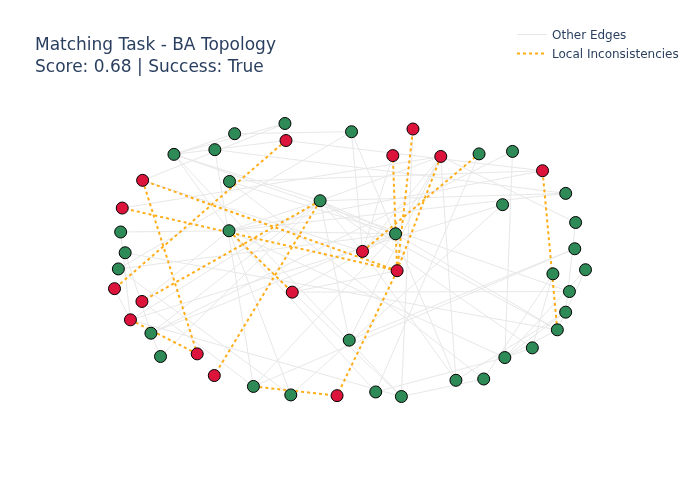
\includegraphics[trim=100 100 90 100,clip,width=0.22\textwidth]{figures/topology/matching_results_20250920_180551_rounds11_gpt-4o-mini_nodes50_langgraph_matching_original.png}}
    \subfloat[SF ($n=100$)]{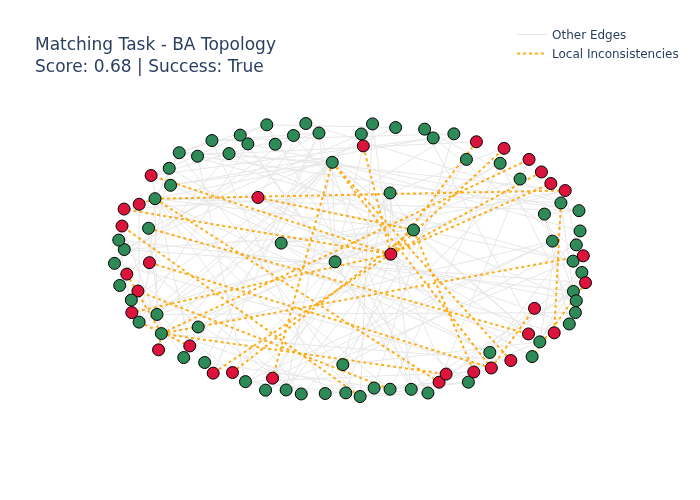
\includegraphics[trim=100 100 90 100,clip,width=0.26\textwidth]{figures/topology/matching_results_20250920_181618_rounds11_gpt-4o-mini_nodes100_langgraph_matching_original.png}}
    \\
    \vspace{2mm}
    % --- DT ---
    \subfloat[DT ($n=4$)]{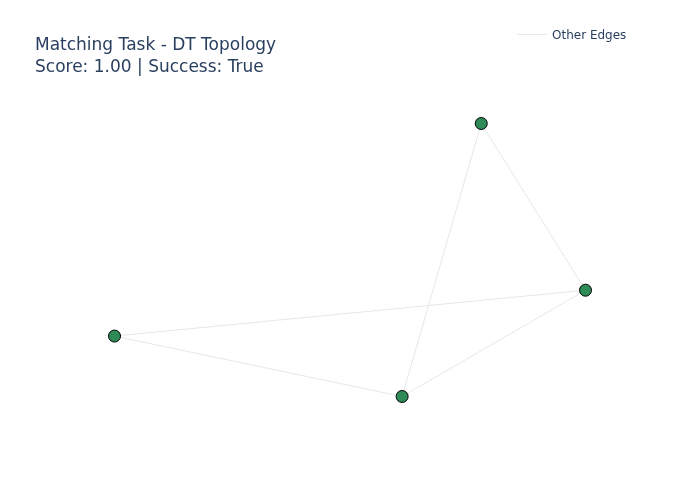
\includegraphics[trim=100 100 90 100,clip,width=0.12\textwidth]{figures/topology/matching_results_20250917_225625_rounds8_gpt-4o-mini_nodes4_langgraph_matching_original.png}}
    \subfloat[DT ($n=8$)]{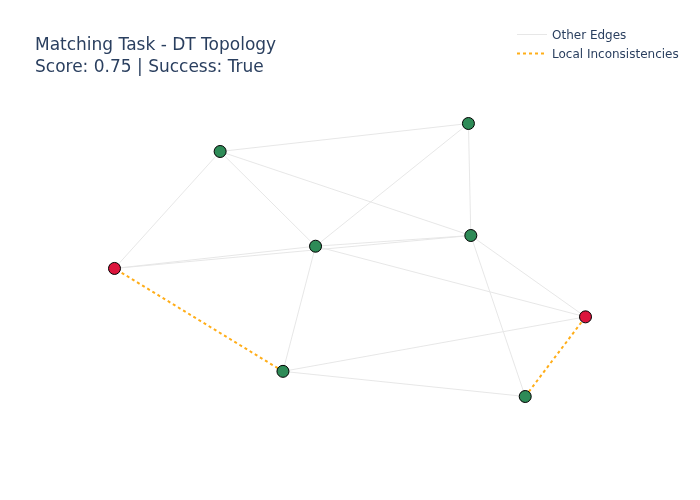
\includegraphics[trim=100 100 90 100,clip,width=0.16\textwidth]{figures/topology/matching_results_20250917_225759_rounds8_gpt-4o-mini_nodes8_langgraph_matching_original.png}}
    \subfloat[DT ($n=16$)]{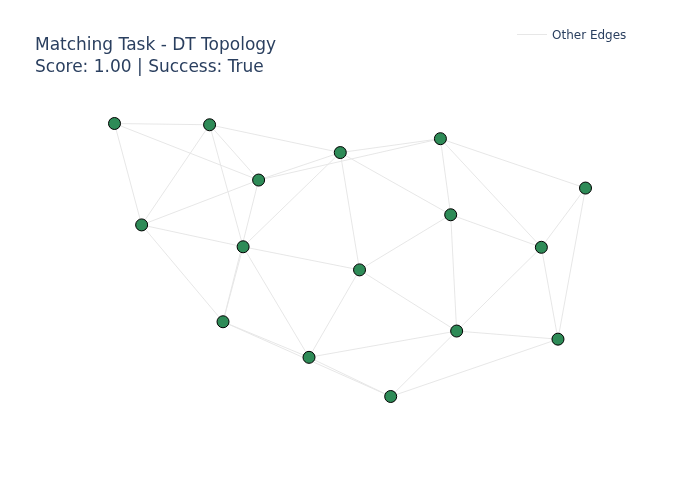
\includegraphics[trim=100 100 90 100,clip,width=0.19\textwidth]{figures/topology/matching_results_20250917_230008_rounds8_gpt-4o-mini_nodes16_langgraph_matching_original.png}}
    \subfloat[DT ($n=50$)]{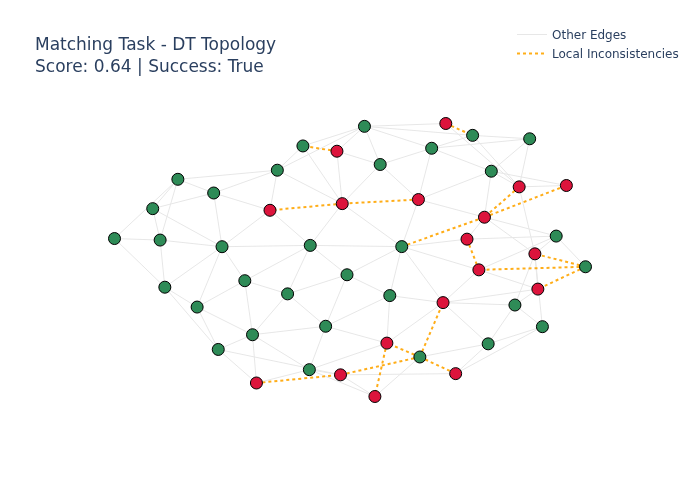
\includegraphics[trim=100 100 90 100,clip,width=0.22\textwidth]{figures/topology/matching_results_20250920_182438_rounds13_gpt-4o-mini_nodes50_langgraph_matching_original.png}}
    \subfloat[DT ($n=100$)]{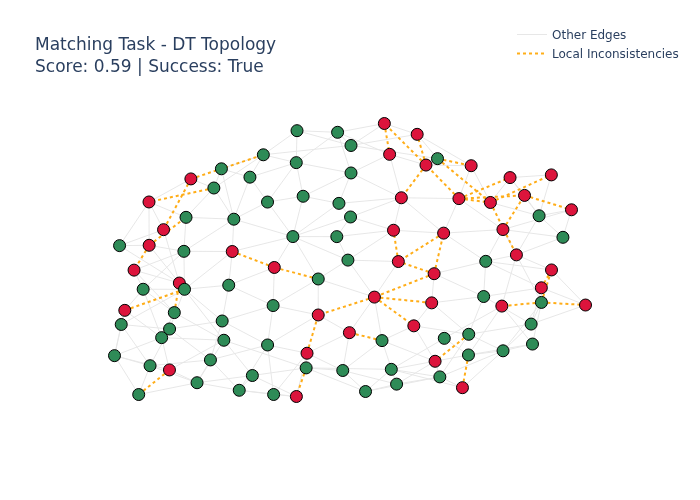
\includegraphics[trim=100 100 90 100,clip,width=0.26\textwidth]{figures/topology/matching_results_20250920_184622_rounds19_gpt-4o-mini_nodes100_langgraph_matching_original.png}}
    \\
    \vspace{2mm}
    % --- SEQUENTIAL ---
    \subfloat[Seq. ($n=4$)]{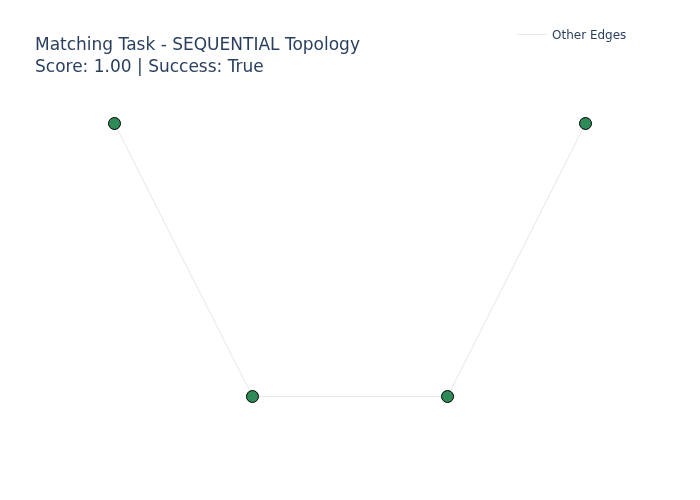
\includegraphics[trim=100 100 90 100,clip,width=0.12\textwidth]{figures/topology/matching_results_20250924_134419_rounds8_gpt-4o-mini_nodes4_crewai-sequential_matching_original.png}}
    \subfloat[Seq. ($n=8$)]{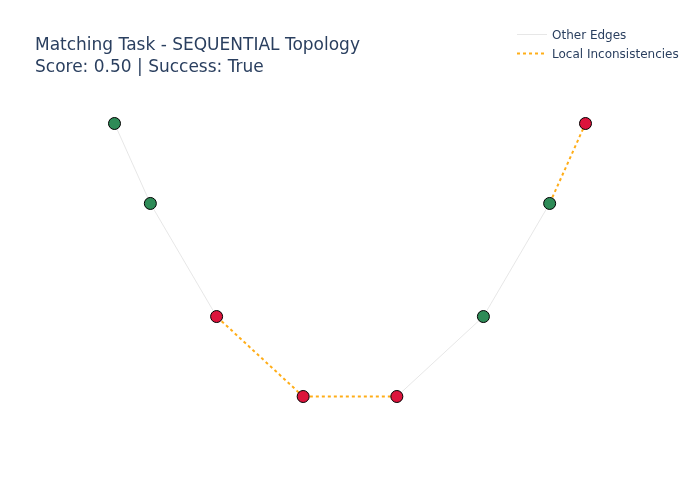
\includegraphics[trim=100 100 90 100,clip,width=0.16\textwidth]{figures/topology/matching_results_20250924_134606_rounds8_gpt-4o-mini_nodes8_crewai-sequential_matching_original.png}}
    \subfloat[Seq. ($n=16$)]{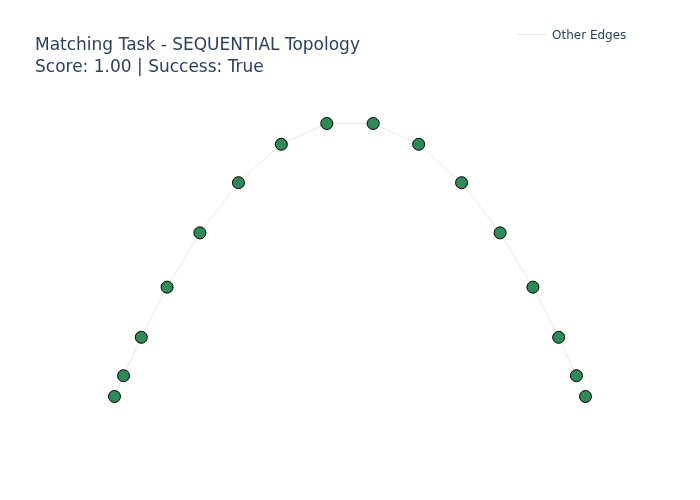
\includegraphics[trim=100 100 90 100,clip,width=0.19\textwidth]{figures/topology/matching_results_20250924_134833_rounds8_gpt-4o-mini_nodes16_crewai-sequential_matching_original.png}}
    \subfloat{\rule{0.22\textwidth}{0pt}} % placeholder without number
    \subfloat{\rule{0.26\textwidth}{0pt}} % placeholder without number
    \\
    \vspace{2mm}
    % --- HIERARCHICAL ---
    \subfloat[Hier. ($n=4$)]{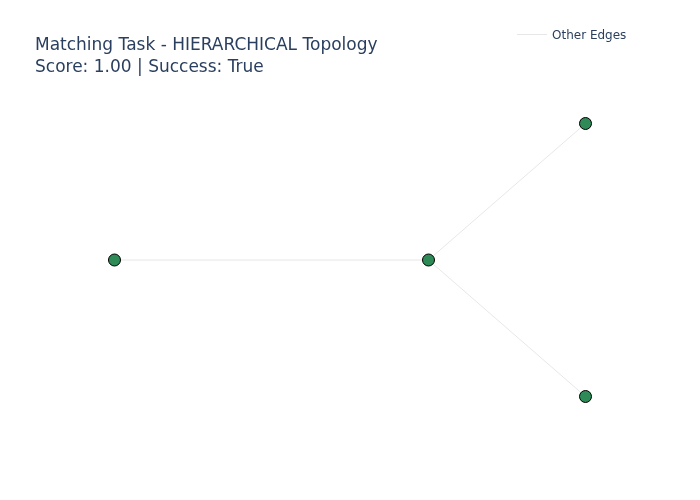
\includegraphics[trim=100 100 90 100,clip,width=0.12\textwidth]{figures/topology/matching_results_20250924_144228_rounds8_gpt-4o-mini_nodes4_crewai-hierarchical_matching_original.png}}
    \subfloat[Hier. ($n=8$)]{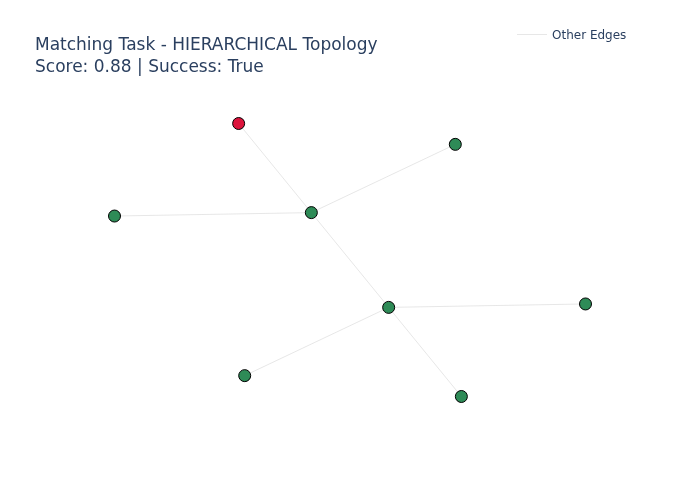
\includegraphics[trim=100 100 90 100,clip,width=0.16\textwidth]{figures/topology/matching_results_20250924_144411_rounds8_gpt-4o-mini_nodes8_crewai-hierarchical_matching_original.png}}
    \subfloat[Hier. ($n=16$)]{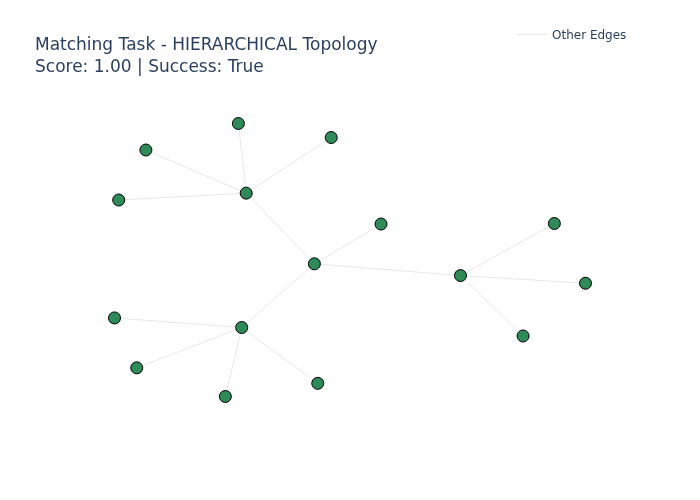
\includegraphics[trim=100 100 90 100,clip,width=0.19\textwidth]{figures/topology/matching_results_20250924_144629_rounds8_gpt-4o-mini_nodes16_crewai-hierarchical_matching_original.png}}
    \subfloat[Hier. ($n=50$)]{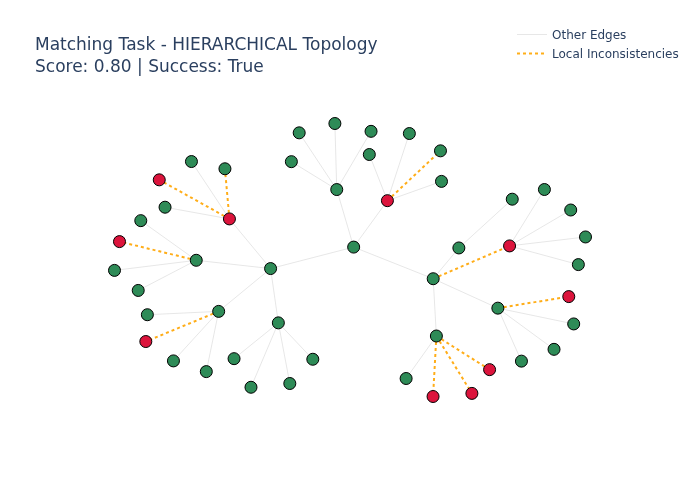
\includegraphics[trim=100 100 90 100,clip,width=0.22\textwidth]{figures/topology/matching_results_20250925_001343_rounds13_gpt-4o-mini_nodes50_crewai-hierarchical_matching_original.png}}
    \subfloat[Hier. ($n=100$)]{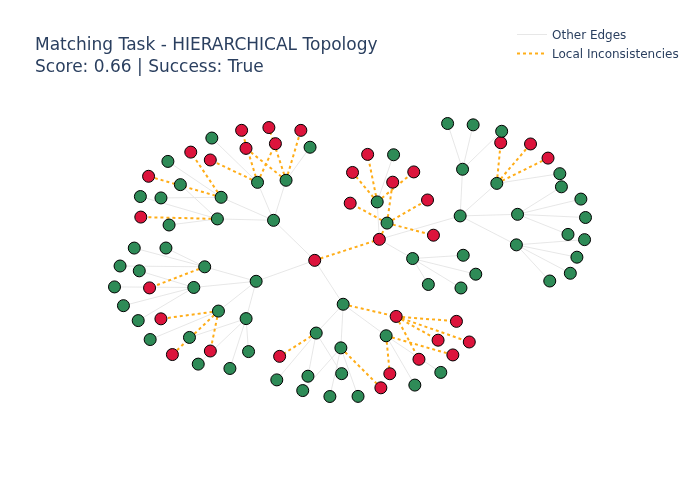
\includegraphics[trim=100 100 90 100,clip,width=0.26\textwidth]{figures/topology/matching_results_20250925_002721_rounds15_gpt-4o-mini_nodes100_crewai-hierarchical_matching_original.png}}
    \\
    \vspace{2mm}
    % --- ALL ---
    \subfloat[All ($n=4$)]{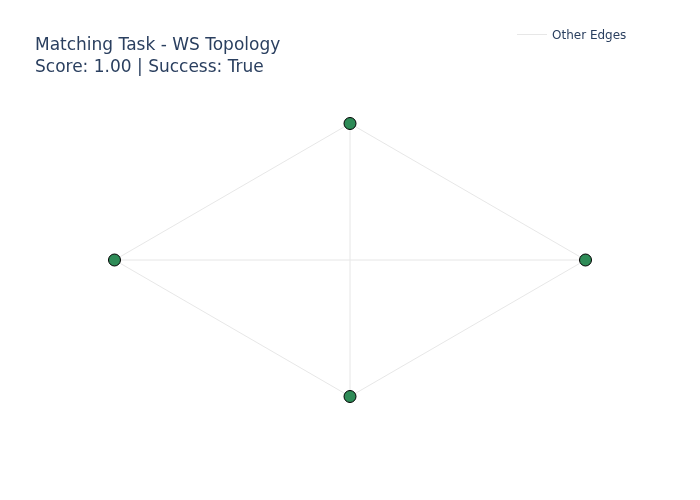
\includegraphics[trim=100 100 90 100,clip,width=0.12\textwidth]{figures/topology/matching_results_20250917_230141_rounds8_gpt-4o-mini_nodes4_concordia_matching_original.png}}
    \subfloat[All ($n=8$)]{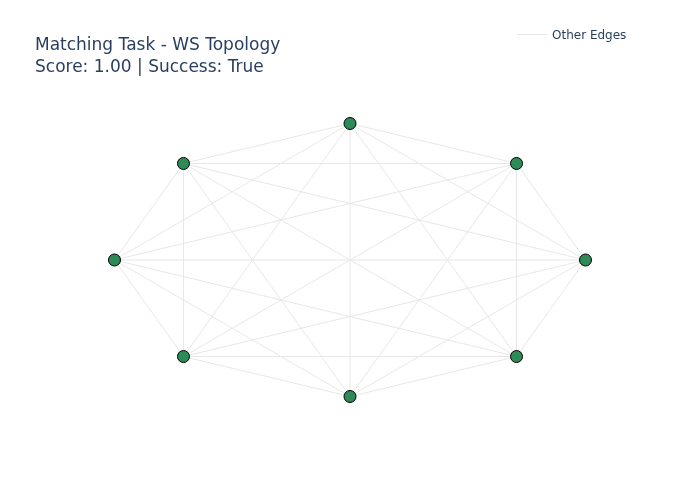
\includegraphics[trim=100 100 90 100,clip,width=0.16\textwidth]{figures/topology/matching_results_20250917_230411_rounds8_gpt-4o-mini_nodes8_concordia_matching_original.png}}
    \subfloat[All ($n=16$)]{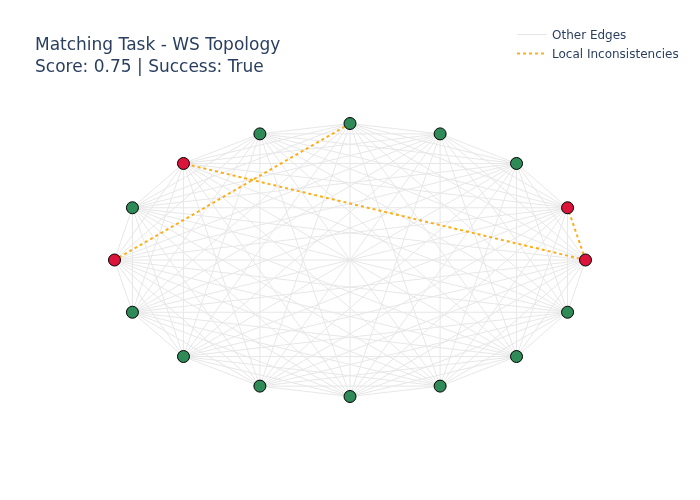
\includegraphics[trim=100 100 90 100,clip,width=0.19\textwidth]{figures/topology/matching_results_20250917_230756_rounds8_gpt-4o-mini_nodes16_concordia_matching_original.png}}
    \subfloat[All ($n=50$)]{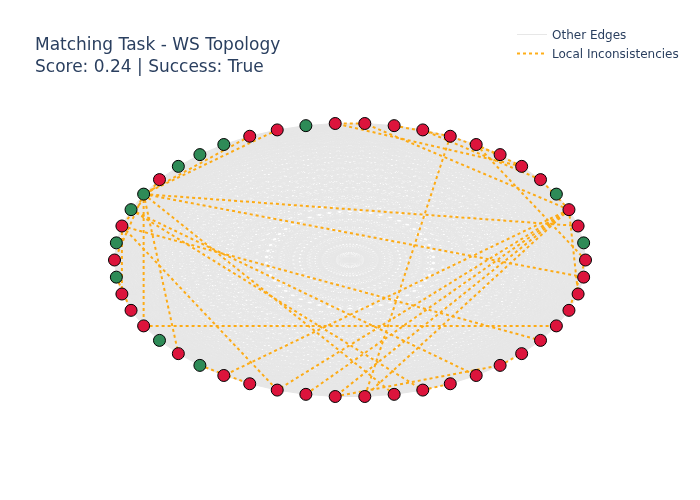
\includegraphics[trim=100 100 90 100,clip,width=0.22\textwidth]{figures/topology/matching_results_20250919_112014_rounds3_gpt-4o-mini_nodes50_concordia_matching_original.png}}
    \subfloat[All ($n=100$)]{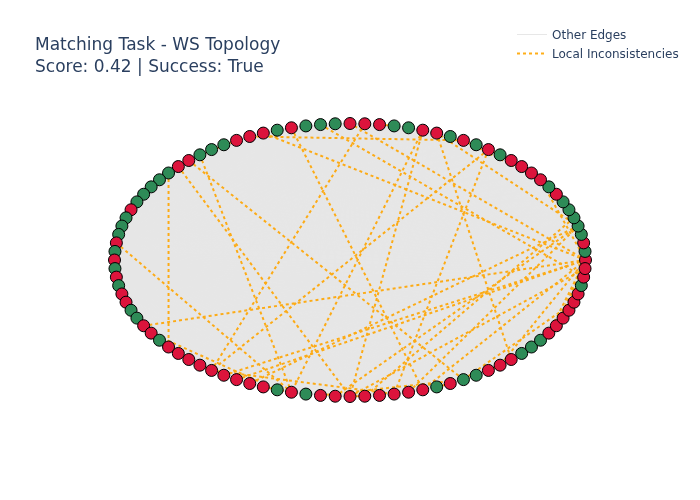
\includegraphics[trim=100 100 90 100,clip,width=0.26\textwidth]{figures/topology/matching_results_20250919_110457_rounds3_gpt-4o-mini_nodes100_concordia_matching_original.png}}
    \\
    \vspace{2mm}
    \caption{Matching experiment outcomes using the \emph{original scoring model}. Each agent selects one of its neighbors (or ``None'') to form a pair. Green nodes denote agents whose selections are locally consistent---that is, they selected a valid neighbor who reciprocated the choice. Red nodes represent agents involved in inconsistencies, such as choosing a non-neighbor, selecting a non-reciprocating partner, or forming idle pairs where both neighbors chose ``None.'' The overall score corresponds to the fraction of locally consistent agents, following the computation described in the text.}


    \label{fig:matching-results}
\end{figure*}


\begin{figure*}[t]
    \centering
    % --- WS ---
    \subfloat[SW ($n=4$)]{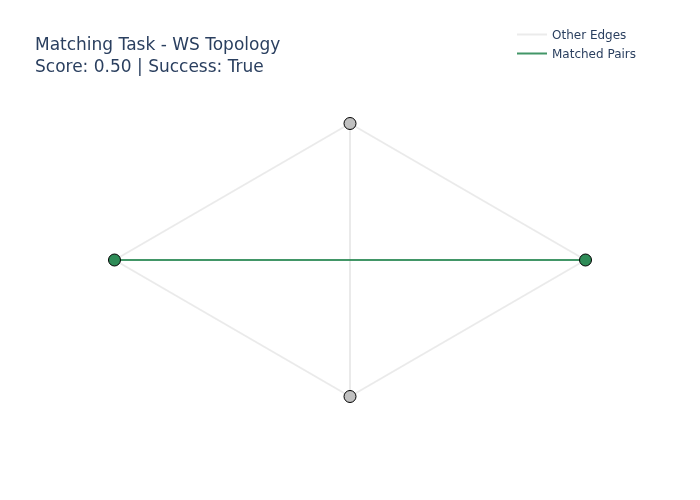
\includegraphics[trim=100 100 90 100,clip,width=0.12\textwidth]{figures/topology/matching_results_20250917_224359_rounds8_gpt-4o-mini_nodes4_langgraph_matching.png}}
    \subfloat[SW ($n=8$)]{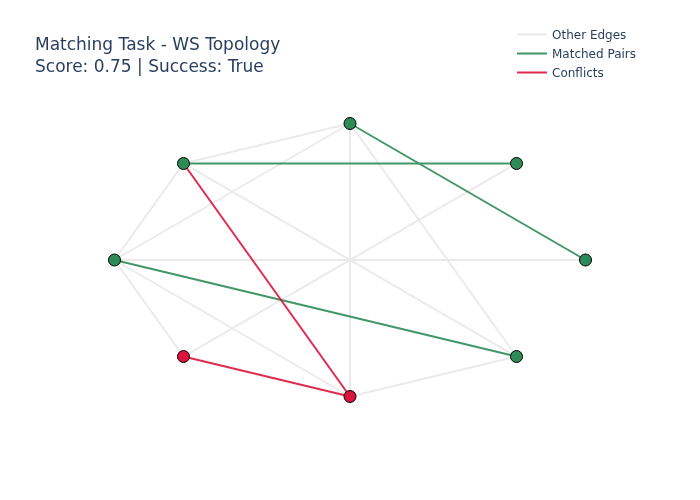
\includegraphics[trim=100 100 90 100,clip,width=0.16\textwidth]{figures/topology/matching_results_20250917_224622_rounds8_gpt-4o-mini_nodes8_langgraph_matching.png}}
    \subfloat[SW ($n=16$)]{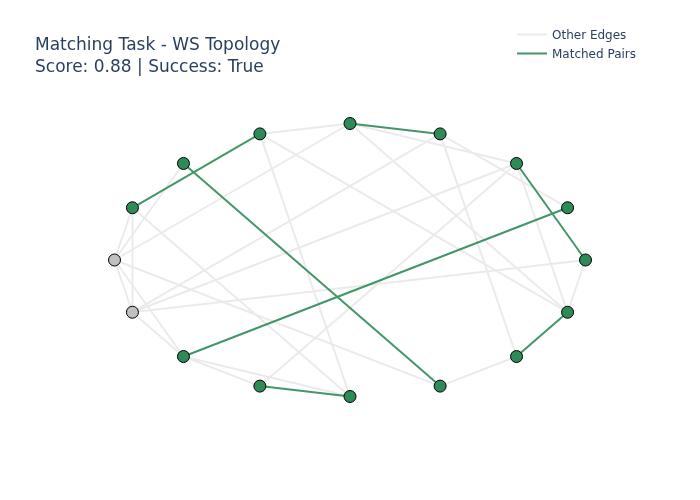
\includegraphics[trim=100 100 90 100,clip,width=0.19\textwidth]{figures/topology/matching_results_20250917_224907_rounds8_gpt-4o-mini_nodes16_langgraph_matching.png}}
    \subfloat[SW ($n=50$)]{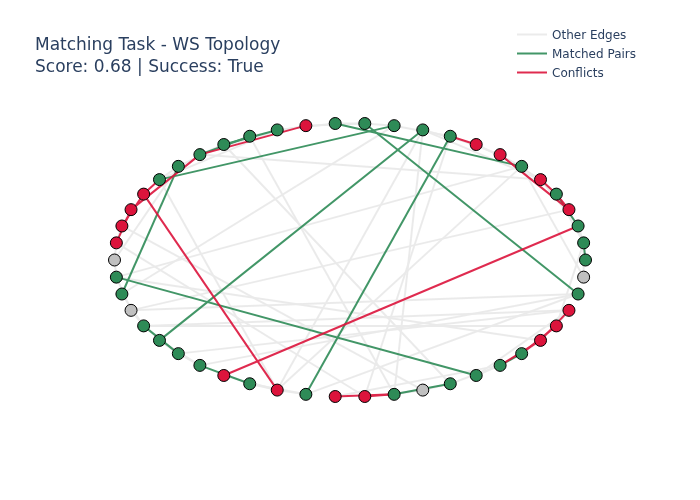
\includegraphics[trim=100 100 90 100,clip,width=0.22\textwidth]{figures/topology/matching_results_20250920_223026_rounds11_gpt-4o-mini_nodes50_langgraph_matching.png}}
    \subfloat[SW ($n=100$)]{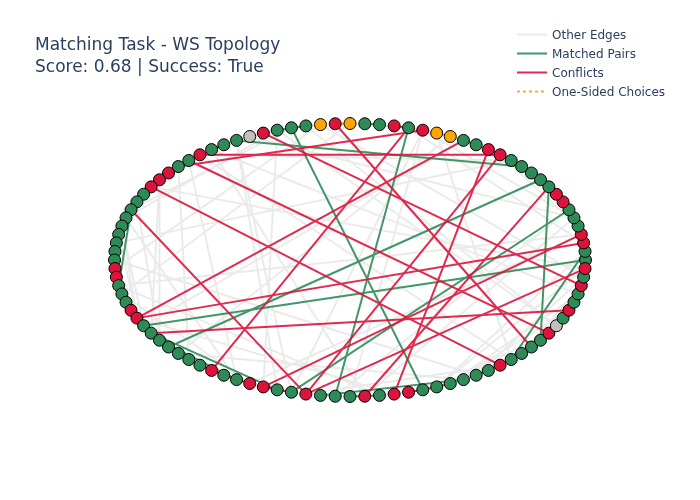
\includegraphics[trim=100 100 90 100,clip,width=0.26\textwidth]{figures/topology/matching_results_20250919_123428_rounds15_gpt-4o-mini_nodes100_langgraph_matching.png}}
    \\
    \vspace{2mm}
    % --- BA ---
    \subfloat[SF ($n=4$)]{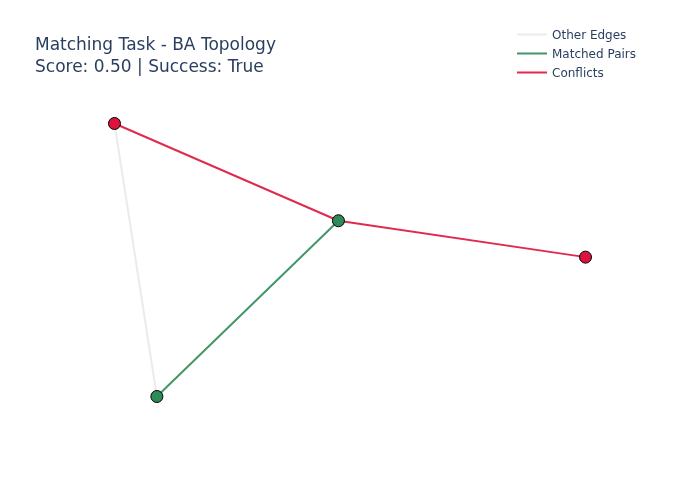
\includegraphics[trim=100 100 90 100,clip,width=0.12\textwidth]{figures/topology/matching_results_20250917_225048_rounds8_gpt-4o-mini_nodes4_langgraph_matching.png}}
    \subfloat[SF ($n=8$)]{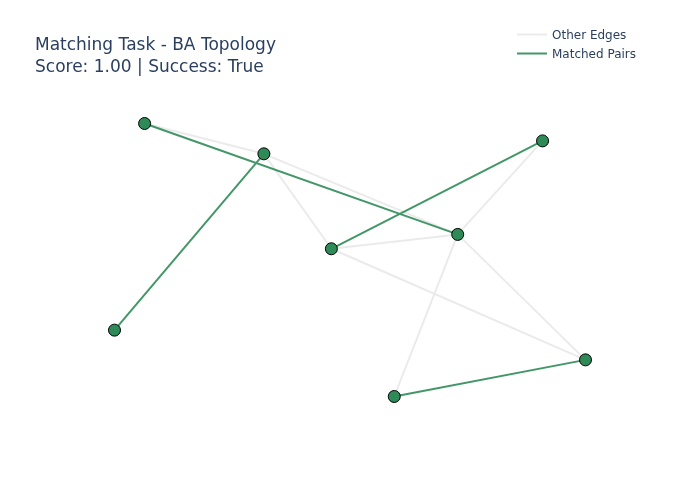
\includegraphics[trim=100 100 90 100,clip,width=0.16\textwidth]{figures/topology/matching_results_20250917_225237_rounds8_gpt-4o-mini_nodes8_langgraph_matching.png}}
    \subfloat[SF ($n=16$)]{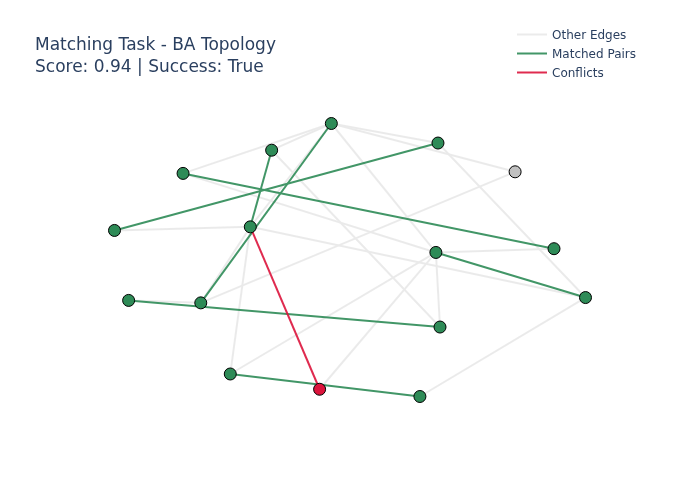
\includegraphics[trim=100 100 90 100,clip,width=0.19\textwidth]{figures/topology/matching_results_20250917_225456_rounds8_gpt-4o-mini_nodes16_langgraph_matching.png}}
    \subfloat[SF ($n=50$)]{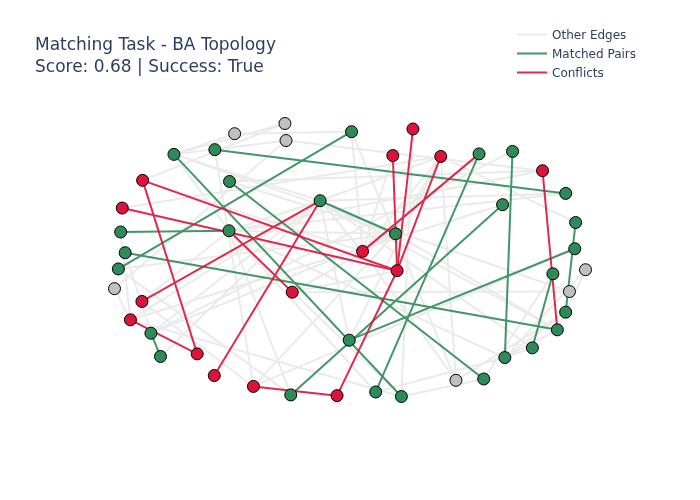
\includegraphics[trim=100 100 90 100,clip,width=0.22\textwidth]{figures/topology/matching_results_20250920_180551_rounds11_gpt-4o-mini_nodes50_langgraph_matching.png}}
    \subfloat[SF ($n=100$)]{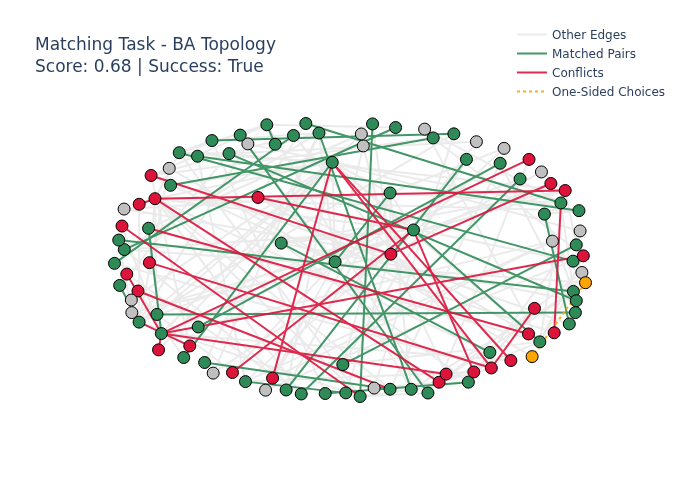
\includegraphics[trim=100 100 90 100,clip,width=0.26\textwidth]{figures/topology/matching_results_20250920_181618_rounds11_gpt-4o-mini_nodes100_langgraph_matching.png}}
    \\
    \vspace{2mm}
    % --- DT ---
    \subfloat[DT ($n=4$)]{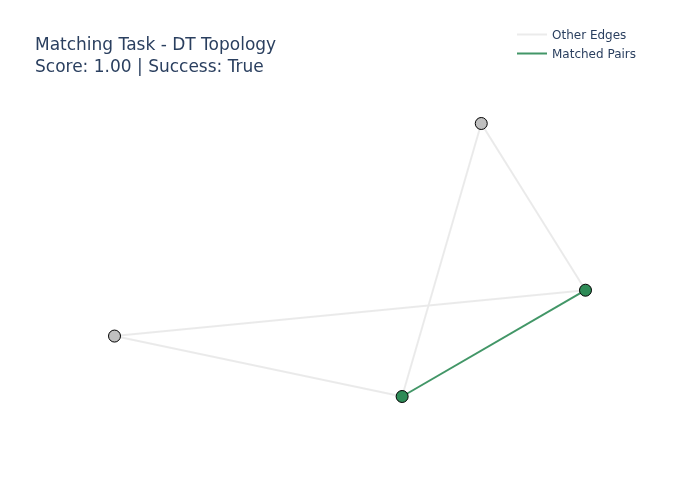
\includegraphics[trim=100 100 90 100,clip,width=0.12\textwidth]{figures/topology/matching_results_20250917_225625_rounds8_gpt-4o-mini_nodes4_langgraph_matching.png}}
    \subfloat[DT ($n=8$)]{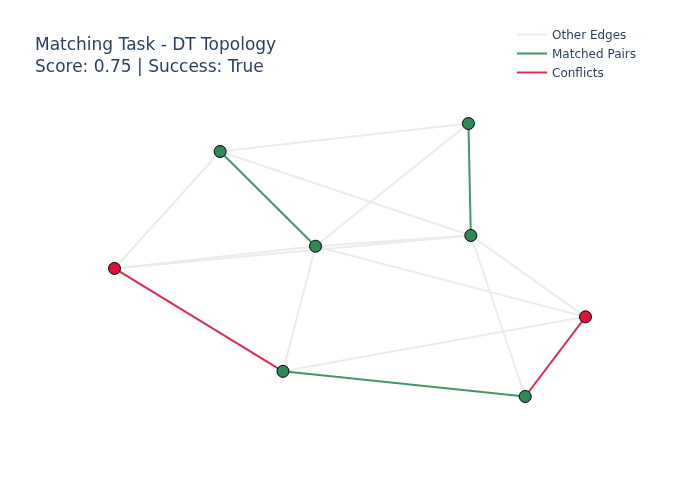
\includegraphics[trim=100 100 90 100,clip,width=0.16\textwidth]{figures/topology/matching_results_20250917_225759_rounds8_gpt-4o-mini_nodes8_langgraph_matching.png}}
    \subfloat[DT ($n=16$)]{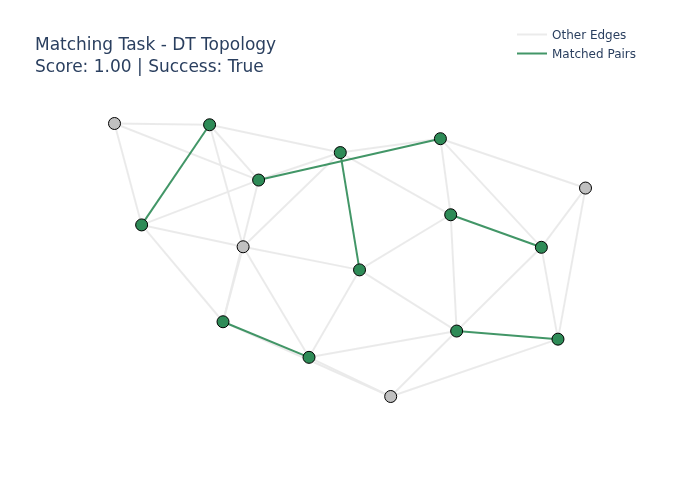
\includegraphics[trim=100 100 90 100,clip,width=0.19\textwidth]{figures/topology/matching_results_20250917_230008_rounds8_gpt-4o-mini_nodes16_langgraph_matching.png}}
    \subfloat[DT ($n=50$)]{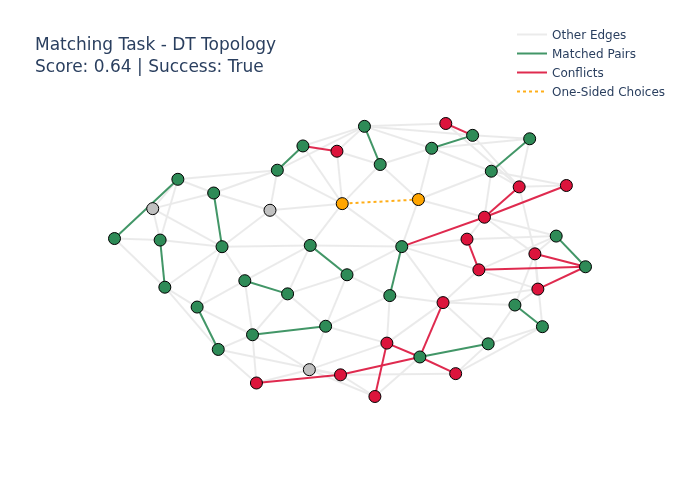
\includegraphics[trim=100 100 90 100,clip,width=0.22\textwidth]{figures/topology/matching_results_20250920_182438_rounds13_gpt-4o-mini_nodes50_langgraph_matching.png}}
    \subfloat[DT ($n=100$)]{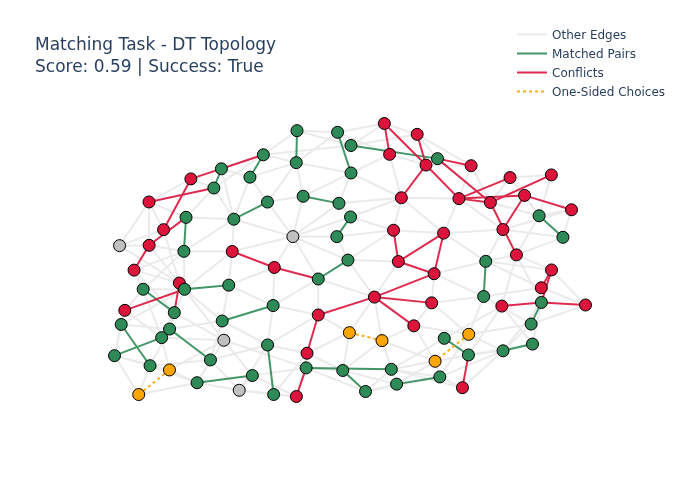
\includegraphics[trim=100 100 90 100,clip,width=0.26\textwidth]{figures/topology/matching_results_20250920_184622_rounds19_gpt-4o-mini_nodes100_langgraph_matching.png}}
    \\
    \vspace{2mm}
    % --- SEQUENTIAL ---
    \subfloat[Seq. ($n=4$)]{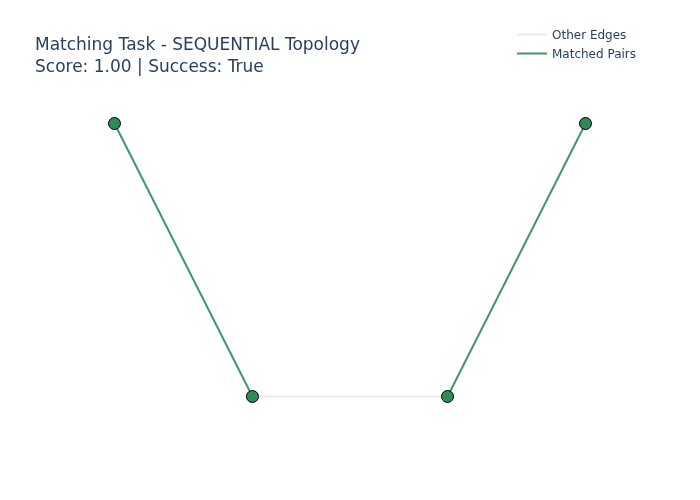
\includegraphics[trim=100 100 90 100,clip,width=0.12\textwidth]{figures/topology/matching_results_20250924_134419_rounds8_gpt-4o-mini_nodes4_crewai-sequential_matching.png}}
    \subfloat[Seq. ($n=8$)]{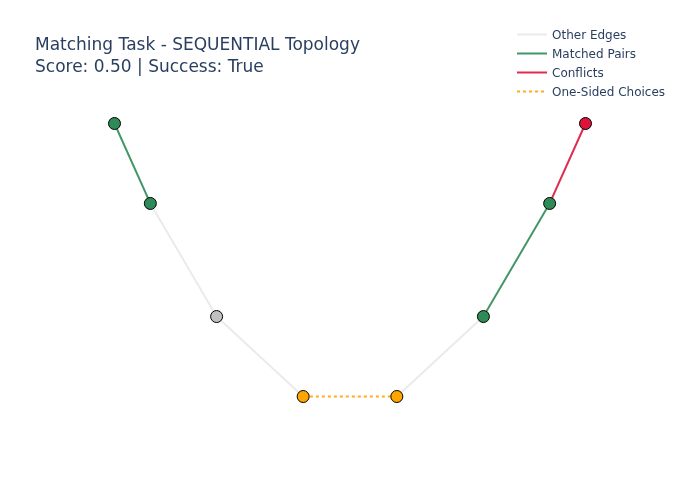
\includegraphics[trim=100 100 90 100,clip,width=0.16\textwidth]{figures/topology/matching_results_20250924_134606_rounds8_gpt-4o-mini_nodes8_crewai-sequential_matching.png}}
    \subfloat[Seq. ($n=16$)]{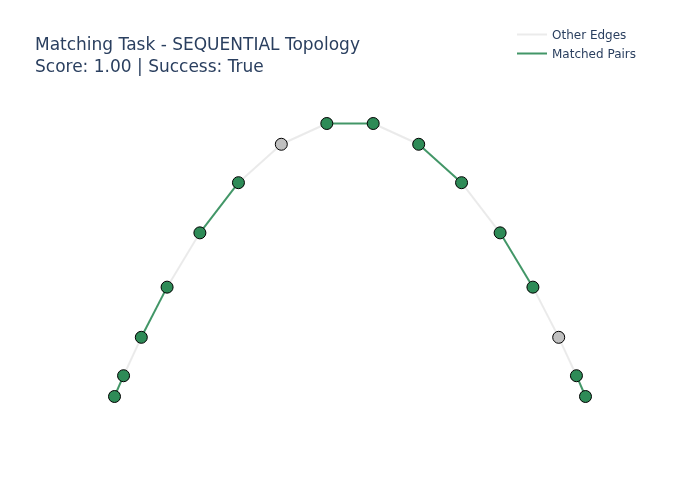
\includegraphics[trim=100 100 90 100,clip,width=0.19\textwidth]{figures/topology/matching_results_20250924_134833_rounds8_gpt-4o-mini_nodes16_crewai-sequential_matching.png}}
    \subfloat{\rule{0.22\textwidth}{0pt}} % placeholder without number
    \subfloat{\rule{0.26\textwidth}{0pt}} % placeholder without number
    \\
    \vspace{2mm}
    % --- HIERARCHICAL ---
    \subfloat[Hier. ($n=4$)]{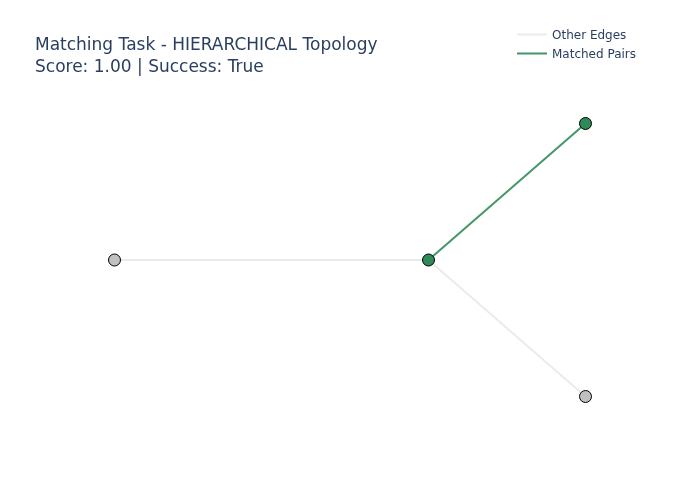
\includegraphics[trim=100 100 90 100,clip,width=0.12\textwidth]{figures/topology/matching_results_20250924_144228_rounds8_gpt-4o-mini_nodes4_crewai-hierarchical_matching.png}}
    \subfloat[Hier. ($n=8$)]{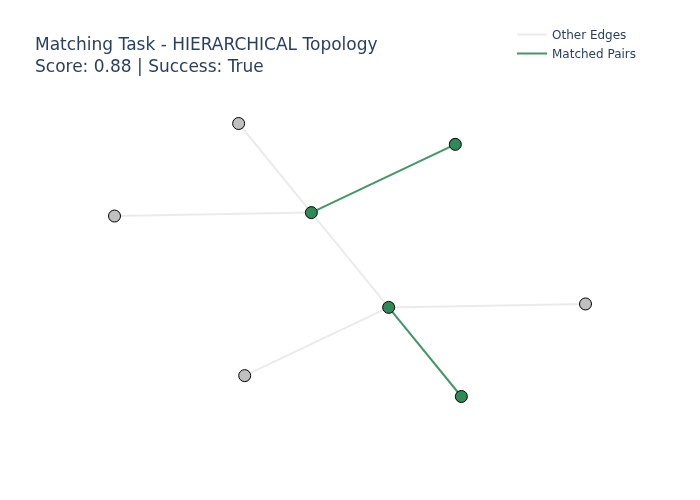
\includegraphics[trim=100 100 90 100,clip,width=0.16\textwidth]{figures/topology/matching_results_20250924_144411_rounds8_gpt-4o-mini_nodes8_crewai-hierarchical_matching.png}}
    \subfloat[Hier. ($n=16$)]{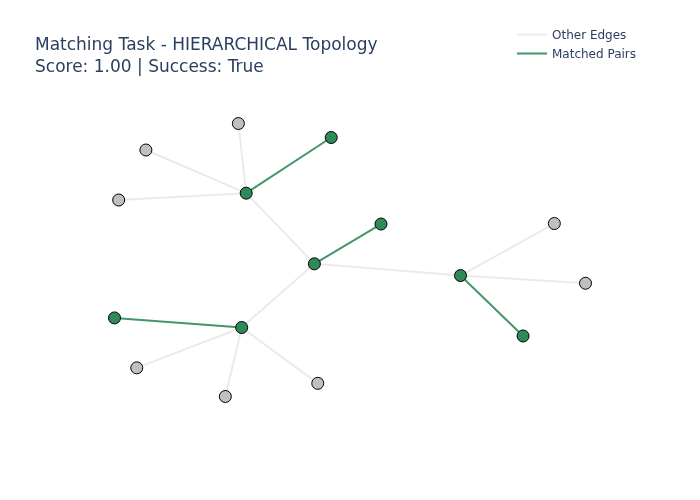
\includegraphics[trim=100 100 90 100,clip,width=0.19\textwidth]{figures/topology/matching_results_20250924_144629_rounds8_gpt-4o-mini_nodes16_crewai-hierarchical_matching.png}}
    \subfloat[Hier. ($n=50$)]{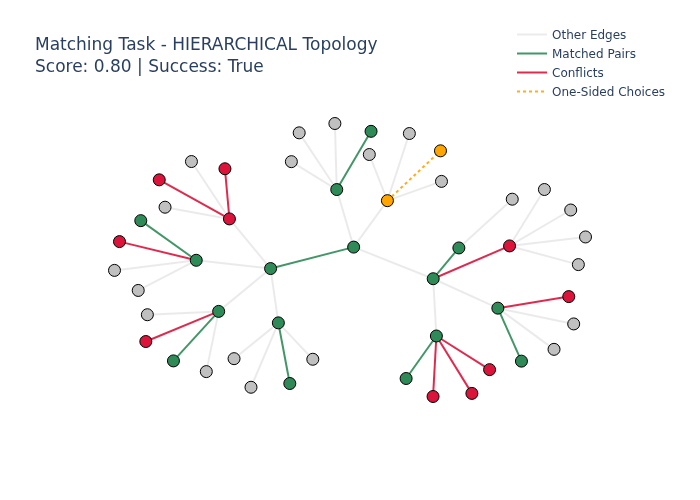
\includegraphics[trim=100 100 90 100,clip,width=0.22\textwidth]{figures/topology/matching_results_20250925_001343_rounds13_gpt-4o-mini_nodes50_crewai-hierarchical_matching.png}}
    \subfloat[Hier. ($n=100$)]{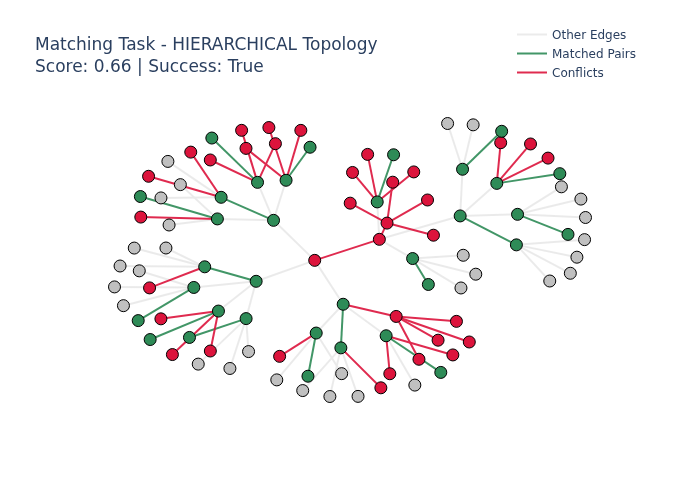
\includegraphics[trim=100 100 90 100,clip,width=0.26\textwidth]{figures/topology/matching_results_20250925_002721_rounds15_gpt-4o-mini_nodes100_crewai-hierarchical_matching.png}}
    \\
    \vspace{2mm}
    % --- ALL ---
    \subfloat[All ($n=4$)]{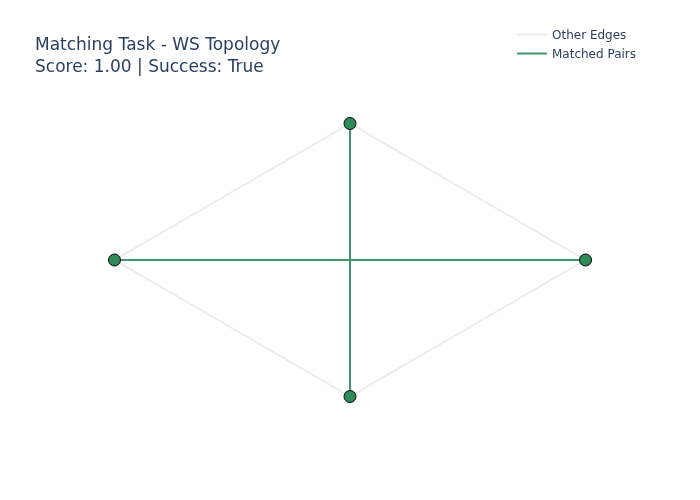
\includegraphics[trim=100 100 90 100,clip,width=0.12\textwidth]{figures/topology/matching_results_20250917_230141_rounds8_gpt-4o-mini_nodes4_concordia_matching.png}}
    \subfloat[All ($n=8$)]{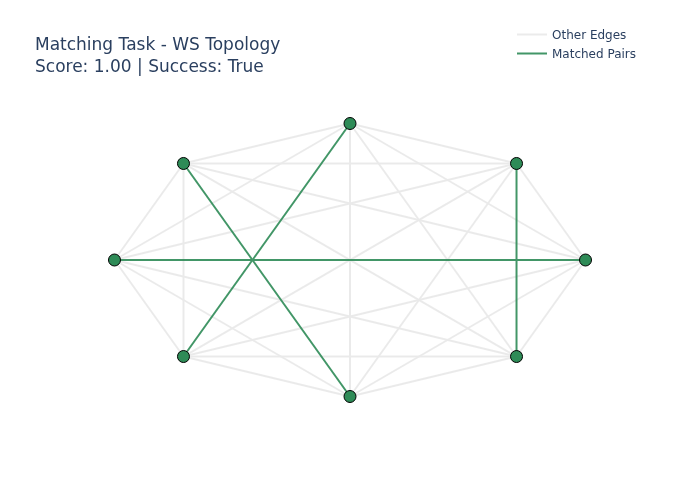
\includegraphics[trim=100 100 90 100,clip,width=0.16\textwidth]{figures/topology/matching_results_20250917_230411_rounds8_gpt-4o-mini_nodes8_concordia_matching.png}}
    \subfloat[All ($n=16$)]{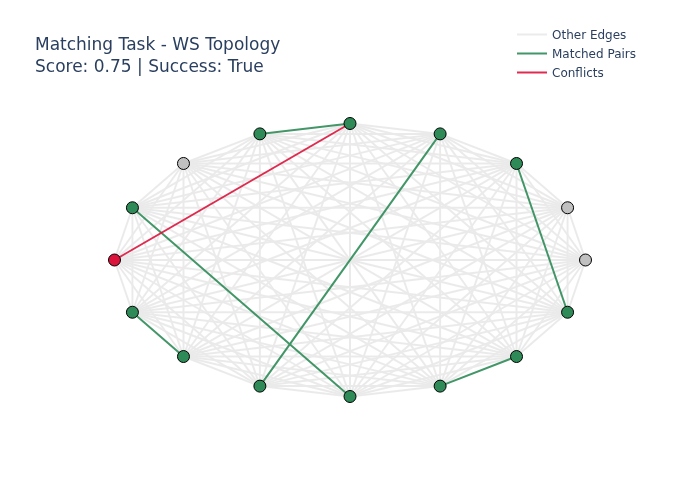
\includegraphics[trim=100 100 90 100,clip,width=0.19\textwidth]{figures/topology/matching_results_20250917_230756_rounds8_gpt-4o-mini_nodes16_concordia_matching.png}}
    \subfloat[All ($n=50$)]{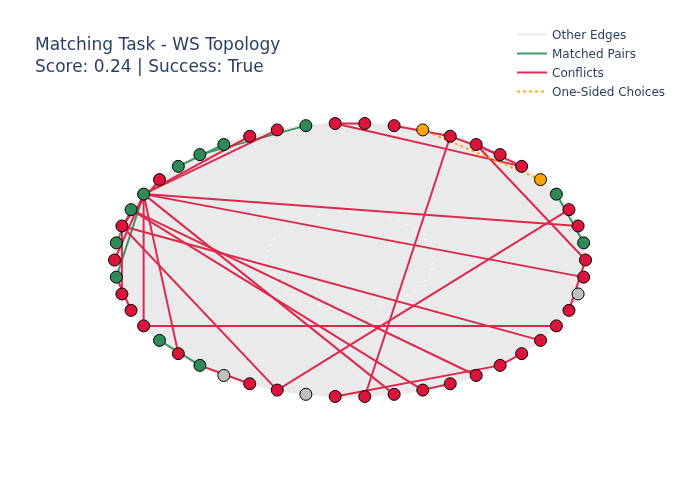
\includegraphics[trim=100 100 90 100,clip,width=0.22\textwidth]{figures/topology/matching_results_20250919_112014_rounds3_gpt-4o-mini_nodes50_concordia_matching.png}}
    \subfloat[All ($n=100$)]{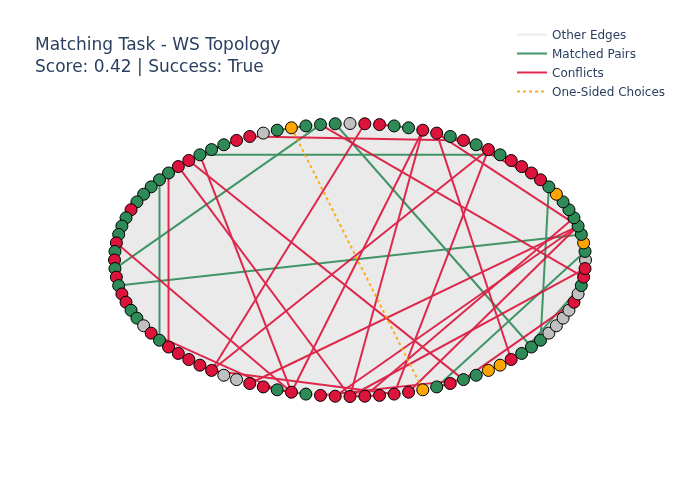
\includegraphics[trim=100 100 90 100,clip,width=0.26\textwidth]{figures/topology/matching_results_20250919_110457_rounds3_gpt-4o-mini_nodes100_concordia_matching.png}}
    \\
    \vspace{2mm}
    \caption{Matching experiment outcomes across different network sizes ($n=4$ to $100$). Each subfigure shows the final pair assignments of agents based on the enhanced local-consistency model. Green edges connect mutually consistent agents whose choices satisfy the neighbor-reciprocation rule; orange dotted edges denote one-sided or invalid selections; and red nodes highlight agents involved in any local inconsistency. Gray edges represent structural links that did not participate in the matching process. This visualization extends the local scoring logic to explicitly reveal consistent and conflicting interactions.}

    \label{fig:matching-results-modified}
\end{figure*}


\input{figures/topology_latex/leader}
\input{figures/topology_latex/vertex}
